% Options for packages loaded elsewhere
% Options for packages loaded elsewhere
\PassOptionsToPackage{unicode}{hyperref}
\PassOptionsToPackage{hyphens}{url}
\PassOptionsToPackage{dvipsnames,svgnames,x11names}{xcolor}
%
\documentclass[
]{agujournal2019}
\usepackage{xcolor}
\usepackage{amsmath,amssymb}
\setcounter{secnumdepth}{5}
\usepackage{iftex}
\ifPDFTeX
  \usepackage[T1]{fontenc}
  \usepackage[utf8]{inputenc}
  \usepackage{textcomp} % provide euro and other symbols
\else % if luatex or xetex
  \usepackage{unicode-math} % this also loads fontspec
  \defaultfontfeatures{Scale=MatchLowercase}
  \defaultfontfeatures[\rmfamily]{Ligatures=TeX,Scale=1}
\fi
\usepackage{lmodern}
\ifPDFTeX\else
  % xetex/luatex font selection
\fi
% Use upquote if available, for straight quotes in verbatim environments
\IfFileExists{upquote.sty}{\usepackage{upquote}}{}
\IfFileExists{microtype.sty}{% use microtype if available
  \usepackage[]{microtype}
  \UseMicrotypeSet[protrusion]{basicmath} % disable protrusion for tt fonts
}{}
\makeatletter
\@ifundefined{KOMAClassName}{% if non-KOMA class
  \IfFileExists{parskip.sty}{%
    \usepackage{parskip}
  }{% else
    \setlength{\parindent}{0pt}
    \setlength{\parskip}{6pt plus 2pt minus 1pt}}
}{% if KOMA class
  \KOMAoptions{parskip=half}}
\makeatother
% Make \paragraph and \subparagraph free-standing
\makeatletter
\ifx\paragraph\undefined\else
  \let\oldparagraph\paragraph
  \renewcommand{\paragraph}{
    \@ifstar
      \xxxParagraphStar
      \xxxParagraphNoStar
  }
  \newcommand{\xxxParagraphStar}[1]{\oldparagraph*{#1}\mbox{}}
  \newcommand{\xxxParagraphNoStar}[1]{\oldparagraph{#1}\mbox{}}
\fi
\ifx\subparagraph\undefined\else
  \let\oldsubparagraph\subparagraph
  \renewcommand{\subparagraph}{
    \@ifstar
      \xxxSubParagraphStar
      \xxxSubParagraphNoStar
  }
  \newcommand{\xxxSubParagraphStar}[1]{\oldsubparagraph*{#1}\mbox{}}
  \newcommand{\xxxSubParagraphNoStar}[1]{\oldsubparagraph{#1}\mbox{}}
\fi
\makeatother


\usepackage{longtable,booktabs,array}
\usepackage{calc} % for calculating minipage widths
% Correct order of tables after \paragraph or \subparagraph
\usepackage{etoolbox}
\makeatletter
\patchcmd\longtable{\par}{\if@noskipsec\mbox{}\fi\par}{}{}
\makeatother
% Allow footnotes in longtable head/foot
\IfFileExists{footnotehyper.sty}{\usepackage{footnotehyper}}{\usepackage{footnote}}
\makesavenoteenv{longtable}
\usepackage{graphicx}
\makeatletter
\newsavebox\pandoc@box
\newcommand*\pandocbounded[1]{% scales image to fit in text height/width
  \sbox\pandoc@box{#1}%
  \Gscale@div\@tempa{\textheight}{\dimexpr\ht\pandoc@box+\dp\pandoc@box\relax}%
  \Gscale@div\@tempb{\linewidth}{\wd\pandoc@box}%
  \ifdim\@tempb\p@<\@tempa\p@\let\@tempa\@tempb\fi% select the smaller of both
  \ifdim\@tempa\p@<\p@\scalebox{\@tempa}{\usebox\pandoc@box}%
  \else\usebox{\pandoc@box}%
  \fi%
}
% Set default figure placement to htbp
\def\fps@figure{htbp}
\makeatother


% definitions for citeproc citations
\NewDocumentCommand\citeproctext{}{}
\NewDocumentCommand\citeproc{mm}{%
  \begingroup\def\citeproctext{#2}\cite{#1}\endgroup}
\makeatletter
 % allow citations to break across lines
 \let\@cite@ofmt\@firstofone
 % avoid brackets around text for \cite:
 \def\@biblabel#1{}
 \def\@cite#1#2{{#1\if@tempswa , #2\fi}}
\makeatother
\newlength{\cslhangindent}
\setlength{\cslhangindent}{1.5em}
\newlength{\csllabelwidth}
\setlength{\csllabelwidth}{3em}
\newenvironment{CSLReferences}[2] % #1 hanging-indent, #2 entry-spacing
 {\begin{list}{}{%
  \setlength{\itemindent}{0pt}
  \setlength{\leftmargin}{0pt}
  \setlength{\parsep}{0pt}
  % turn on hanging indent if param 1 is 1
  \ifodd #1
   \setlength{\leftmargin}{\cslhangindent}
   \setlength{\itemindent}{-1\cslhangindent}
  \fi
  % set entry spacing
  \setlength{\itemsep}{#2\baselineskip}}}
 {\end{list}}
\usepackage{calc}
\newcommand{\CSLBlock}[1]{\hfill\break\parbox[t]{\linewidth}{\strut\ignorespaces#1\strut}}
\newcommand{\CSLLeftMargin}[1]{\parbox[t]{\csllabelwidth}{\strut#1\strut}}
\newcommand{\CSLRightInline}[1]{\parbox[t]{\linewidth - \csllabelwidth}{\strut#1\strut}}
\newcommand{\CSLIndent}[1]{\hspace{\cslhangindent}#1}



\setlength{\emergencystretch}{3em} % prevent overfull lines

\providecommand{\tightlist}{%
  \setlength{\itemsep}{0pt}\setlength{\parskip}{0pt}}



 


\usepackage{url} %this package should fix any errors with URLs in refs.
\usepackage{lineno}
\usepackage[inline]{trackchanges} %for better track changes. finalnew option will compile document with changes incorporated.
\usepackage{soul}
\linenumbers
\makeatletter
\@ifpackageloaded{float}{}{\usepackage{float}}
\floatstyle{plain}
\@ifundefined{c@chapter}{\newfloat{appfig}{h}{loappfig}}{\newfloat{appfig}{h}{loappfig}[chapter]}
\floatname{appfig}{A}
\newcommand*\listofappfigs{\listof{appfig}{List of Appendix Figures}}
\makeatother
\makeatletter
\@ifpackageloaded{caption}{}{\usepackage{caption}}
\AtBeginDocument{%
\ifdefined\contentsname
  \renewcommand*\contentsname{Table of contents}
\else
  \newcommand\contentsname{Table of contents}
\fi
\ifdefined\listfigurename
  \renewcommand*\listfigurename{List of Figures}
\else
  \newcommand\listfigurename{List of Figures}
\fi
\ifdefined\listtablename
  \renewcommand*\listtablename{List of Tables}
\else
  \newcommand\listtablename{List of Tables}
\fi
\ifdefined\figurename
  \renewcommand*\figurename{Figure}
\else
  \newcommand\figurename{Figure}
\fi
\ifdefined\tablename
  \renewcommand*\tablename{Table}
\else
  \newcommand\tablename{Table}
\fi
}
\@ifpackageloaded{float}{}{\usepackage{float}}
\floatstyle{ruled}
\@ifundefined{c@chapter}{\newfloat{codelisting}{h}{lop}}{\newfloat{codelisting}{h}{lop}[chapter]}
\floatname{codelisting}{Listing}
\newcommand*\listoflistings{\listof{codelisting}{List of Listings}}
\makeatother
\makeatletter
\makeatother
\makeatletter
\@ifpackageloaded{caption}{}{\usepackage{caption}}
\@ifpackageloaded{subcaption}{}{\usepackage{subcaption}}
\makeatother
\usepackage{bookmark}
\IfFileExists{xurl.sty}{\usepackage{xurl}}{} % add URL line breaks if available
\urlstyle{same}
\hypersetup{
  pdftitle={Arizona Random Forest Flood Mapping},
  pdfauthor={Travis Zalesky},
  pdfkeywords={Arizona, Flood, Federal Emergency Management
Administration, Random Forest, Machine Learning},
  colorlinks=true,
  linkcolor={blue},
  filecolor={Maroon},
  citecolor={Blue},
  urlcolor={Blue},
  pdfcreator={LaTeX via pandoc}}



\draftfalse

\begin{document}
\title{Arizona Random Forest Flood Mapping}

\authors{Travis Zalesky\affil{1}}
\affiliation{1}{University of Arizona, }
\correspondingauthor{Travis Zalesky}{travisz@arizona.edu}


\begin{abstract}
Federal Emergency Management Administration 100-year flood risk maps are
expanded across the state of Arizona using a random forest, machine
learning classification utilizing eight topographic explanatory
variables.
\end{abstract}

\section*{Plain Language Summary}
Flood mapping across Arizona.




\section{Background}\label{background}

A critical component of the Arizona Department of Water Resources (ADWR)
Tri-University Recharge Project (TURP, a.k.a ATUR) is a state wide
assessment of flooding potential. Initial efforts focused on a
traditional suitability analysis approach, using the analytical
hierarchy process (AHP) for multi-criterion decision making, largely
based on the work by Aloui et al. (2024). These methods saw initial
success, and are continuing to be developed and refined. However, it
became apparent that there were a number of shortcomings inherent in
this analysis which are not easily addressed.

Firstly, the results of such an analysis are intrinsically linked to the
data layers used, and the weighting schema determined by the AHP. As
additional data sets became available, and alternate weighting schemas
were tested we generated multiple versions of mapped flood potential
which did not necessarily agree with each other. In the absence of high
quality ground-truthed data it was difficult to validate these results
and it was not clear to the project team which version was the best.
This underscores the need for expert involvement at every stage in these
AHP based analysis. While there is a wealth of hydrological expertise
within the larger ATUR project, method development and implementation
has largely been conducted by a GIS technician with marginal hydrologic
knowledge, and it has been difficult to foster sustained buy-in from
team members on this portion of the project.

Furthermore, it was extremely difficult to develop a single generalized
model that would be effective across the whole state. Because of the
wide array of ecological and geologic conditions that are present across
the state variables that are important for flood risk in one region may
not apply in other regions. Lastly, even if these technical issues could
be overcome, there was still gaps in the input data layers, resulting in
unclassified regions.

While the traditional suitability analysis methods of assessing flood
potential is still valuable to the project, and will be retained and
developed further, the reality of these challenges lead us to reevaluate
our overall approach and consider alternate methods. Work by Mudashiru
et al. (2021) summarized the various methods used by other researchers
in this field, which includes AHP based methods as well as physical
modeling and machine learning applications. The machine learning methods
utilized by Tehrany et al. (2019) appeared to be particularly relevant
and applicable. In particular, their use of topographic data
\textbf{only} was particularly intriguing. These data sets are fully
calculable from a digital elevation model (DEM), which are readily
available, easily accessible, and have full coverage over the study
area. These findings lead to a renewed initiative to apply a machine
learning based method towards the objective of a state wide flooding
potential map.

\section{Data \& Methods}\label{sec-data-methods}

All explanatory variables for the model were derived from the NASA
Shuttle Radar Topography Mission (SRTM) 30-m DEM. Slope, aspect,
curvature, stream power index (SPI), topographic wetness index (TWI),
and sediment transport index (STI) were all calculated in ArcGIS Pro
(3.4.3). Slope, aspect and curvature were calculated using the Surface
Parameters tool (Spatial Analyst). SPI, TWI, and STI were calculated as
per Tehrany et al. (2019) using the Raster Calculator according to
Equations \ref{eq-spi}-\ref{eq-sti}

\begin{equation}\phantomsection\label{eq-spi}{
SPI = A_s * tan(ß)
}\end{equation}

\begin{equation}\phantomsection\label{eq-twi}{
TWI = ln(A_s / tan(ß))
}\end{equation}

\begin{equation}\phantomsection\label{eq-sti}{
STI = (A_s / 22.13)^{0.6} * (sin(ß)/0.0896)^{1.3}
}\end{equation}

where A\textsubscript{s} is catchment area (m) and ß is slope (radians).

Similarly, Topographic Roughness Index (TRI) was calculated as per
Tehrany et al. (2019) using a custom R (4.4.1) function with the package
terra (1.7-78) according to Equation~\ref{eq-tri}

\begin{equation}\phantomsection\label{eq-tri}{
TRI = \left[ \sum (χ_{ij} - χ_{00})^2 \right] ^{0.5}
}\end{equation}

where χ\textsubscript{ij} is the elevation at coordinates (i, j) and
χ\textsubscript{00} is the elevation at coordinates (0, 0) for a 3x3
focal neighborhood. The code used to calculate TRI is available on
\href{https://github.com/travisz09/TopographicRoughnessIndex}{GitHub}.

Flood data used for training the model was obtained from the Federal
Emergency Management Administration (FEMA) National Flood Hazards Layer,
which provides 100-year flood maps for many areas of the US. The data
was manually downloaded for each county in AZ from the FEMA
\href{https://hazards-fema.maps.arcgis.com/apps/webappviewer/index.html?id=8b0adb51996444d4879338b5529aa9cd}{data
viewer} (accessed 3/15/2025). Data layers were merged in ArcGIS Pro
(3.4.3), and the vector data was converted to a raster with a 10 m
resolution. Additionally, the FEMA data was reclassified to a binary
output, either flooded or not flooded (during a 100-year flood event),
eliminating details such as survey methods and flow depth.

The machine learning model was performed in Google Earth Engine (GEE).
The SRTM elevation data was access and clipped to the study area
natively through GEE servers, all other data layers, including the study
area shapefile, were uploaded as an asset to GEE prior to model
implementation.

Prior to modeling, the collinearity of the explanatory variables was
explored using a series of pair-wise linear regression plots shown in
Figures A\ref{appfig-floodElev}-A\ref{appfig-triSti}. For collinearity
analysis 5,000 points were randomly sampled across the study area, the
maximum number of points which can be plotted in GEE. The collinearity
of each pair-wise regression is summarized visually in
Figure~\ref{fig-Rsquared} using the R-squared statistic of each
comparison.

\begin{figure}

\centering{

\pandocbounded{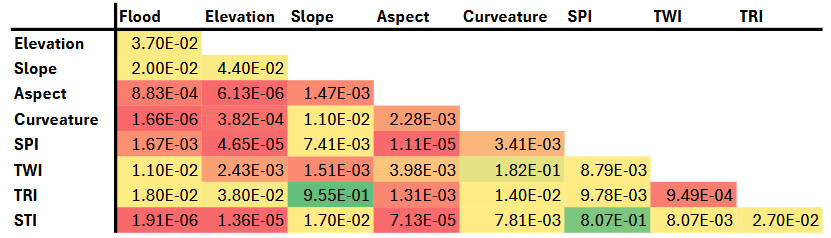
\includegraphics[keepaspectratio]{images/CorrelationMatrix.png}}

}

\caption{\label{fig-Rsquared}Color coded R-squared statistic for each
pair-wise linear regression (green = high, red = low), representing the
collinearity of each variable used for modeling.}

\end{figure}%

\section{Conclusion}\label{conclusion}

\section*{References}\label{references}
\addcontentsline{toc}{section}{References}

\phantomsection\label{refs}
\begin{CSLReferences}{1}{0}
\vspace{1em}

\bibitem[\citeproctext]{ref-Aloui_Zghibi_Mazzoni_Elomri_Al-Ansari_2024}
Aloui, S., Zghibi, A., Mazzoni, A., Elomri, A., \& Al-Ansari, T. (2024).
\emph{Identifying suitable zones for integrated aquifer recharge and
flood control in arid qatar using GIS-based multi-criteria
decision-making}. \emph{25}, 101137.
\url{https://doi.org/10.1016/j.gsd.2024.101137}

\bibitem[\citeproctext]{ref-Mudashiru_Sabtu_Abustan_Balogun_2021}
Mudashiru, R. B., Sabtu, N., Abustan, I., \& Balogun, W. (2021). Flood
hazard mapping methods: A review. \emph{Journal of Hydrology},
\emph{603}, 126846. \url{https://doi.org/10.1016/j.jhydrol.2021.126846}

\bibitem[\citeproctext]{ref-Tehrany_Jones_Shabani_2019}
Tehrany, M. S., Jones, S., \& Shabani, F. (2019). Identifying the
essential flood conditioning factors for flood prone area mapping using
machine learning techniques. \emph{CATENA}, \emph{175}, 174--192.
\url{https://doi.org/10.1016/j.catena.2018.12.011}

\end{CSLReferences}

\section{Appendix}\label{appendix}

\textbf{Flooding}

\begin{appfig}

\centering{

\pandocbounded{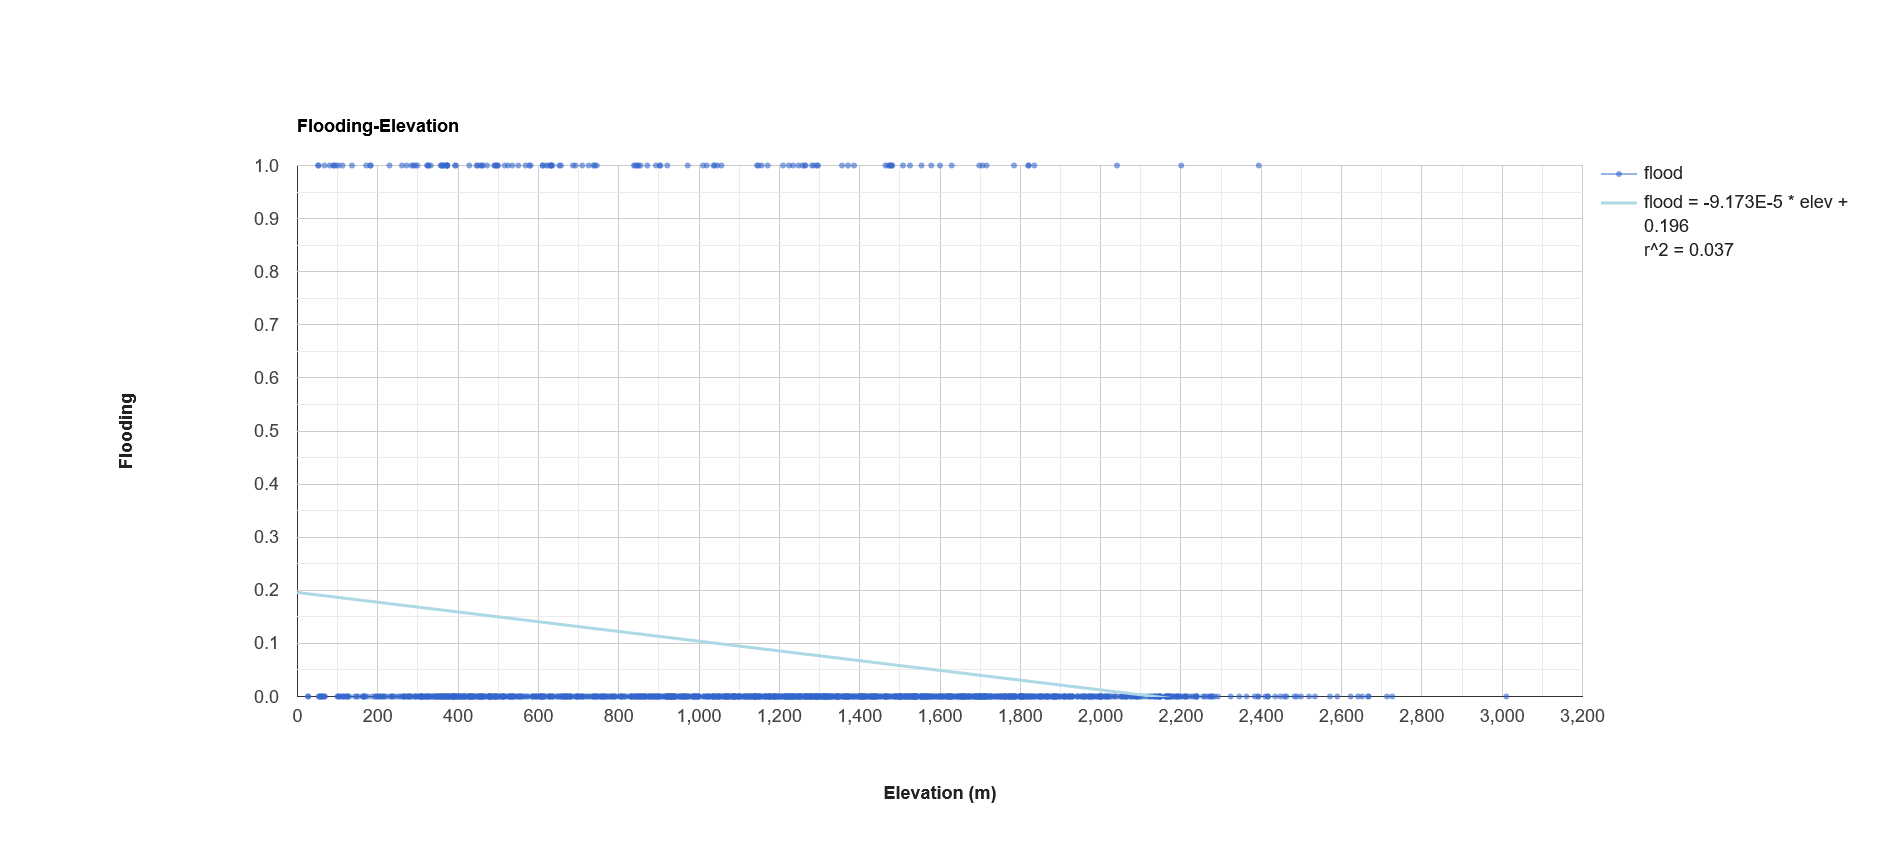
\includegraphics[keepaspectratio]{images/Collinearity/flood-elev.png}}

}

\caption{\label{appfig-floodElev}Linear regression analysis of flood
risk (binary) and elevation (m) for 5,000 randomly sampled points across
the full study area, encompassing Arizona.}

\end{appfig}%

\begin{appfig}

\centering{

\pandocbounded{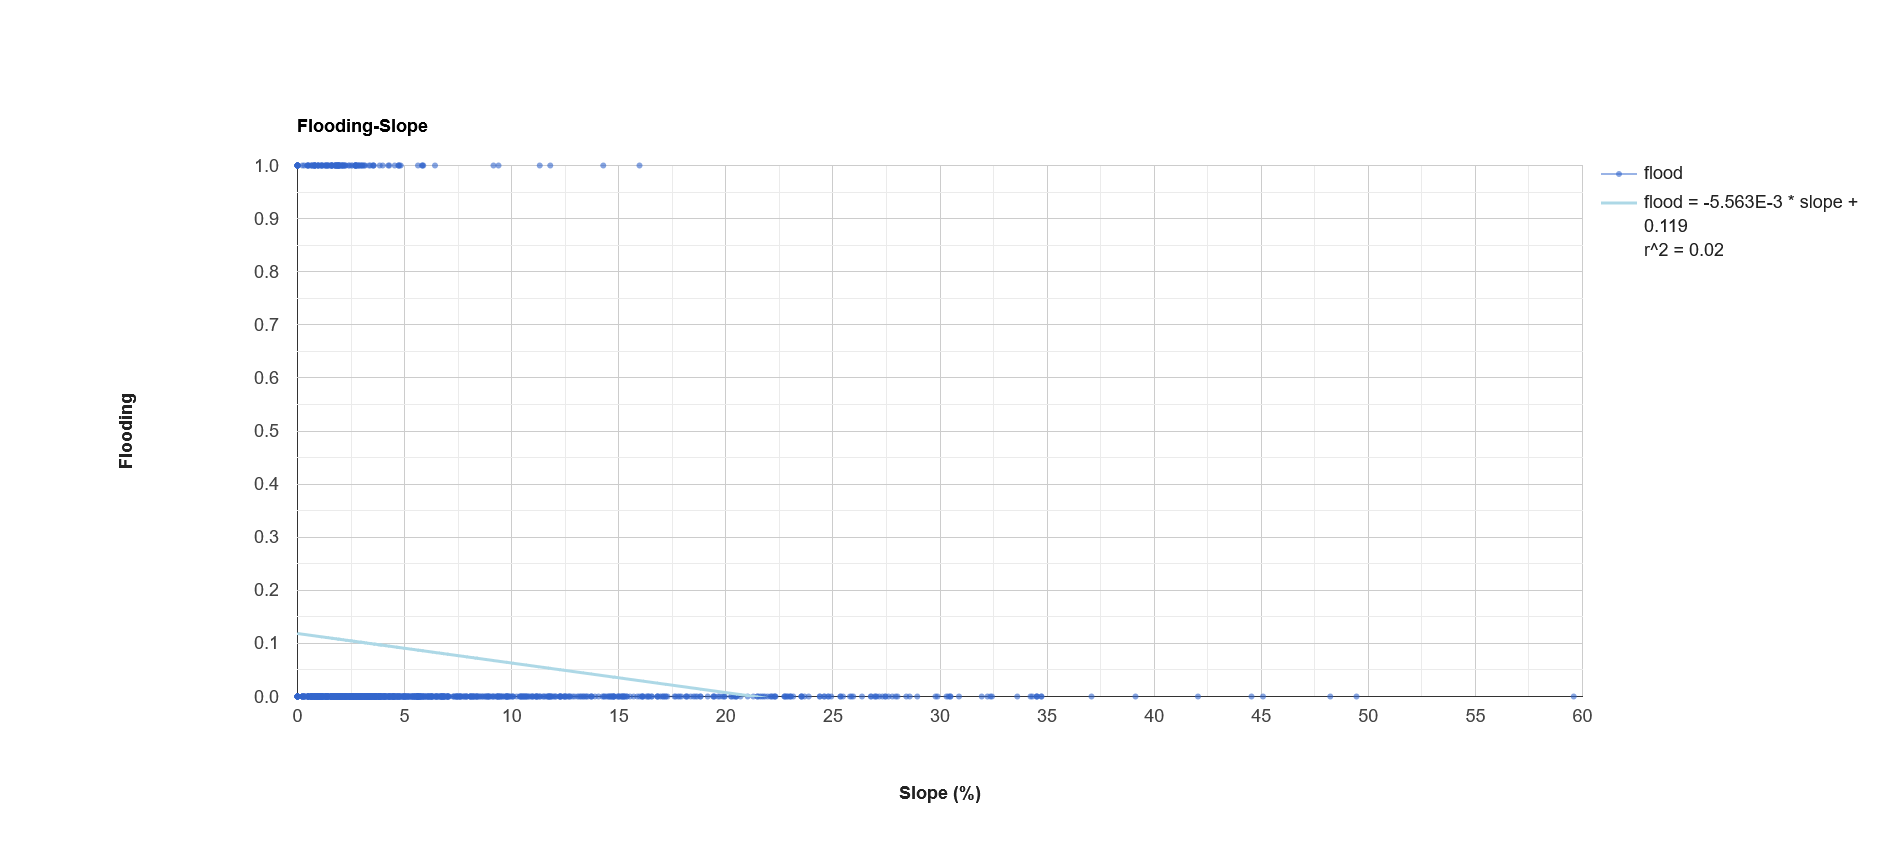
\includegraphics[keepaspectratio]{images/Collinearity/flood-slope.png}}

}

\caption{\label{appfig-floodSlope}Linear regression analysis of flood
risk (binary) and slope (°) for 5,000 randomly sampled points across the
full study area, encompassing Arizona.}

\end{appfig}%

\begin{appfig}

\centering{

\pandocbounded{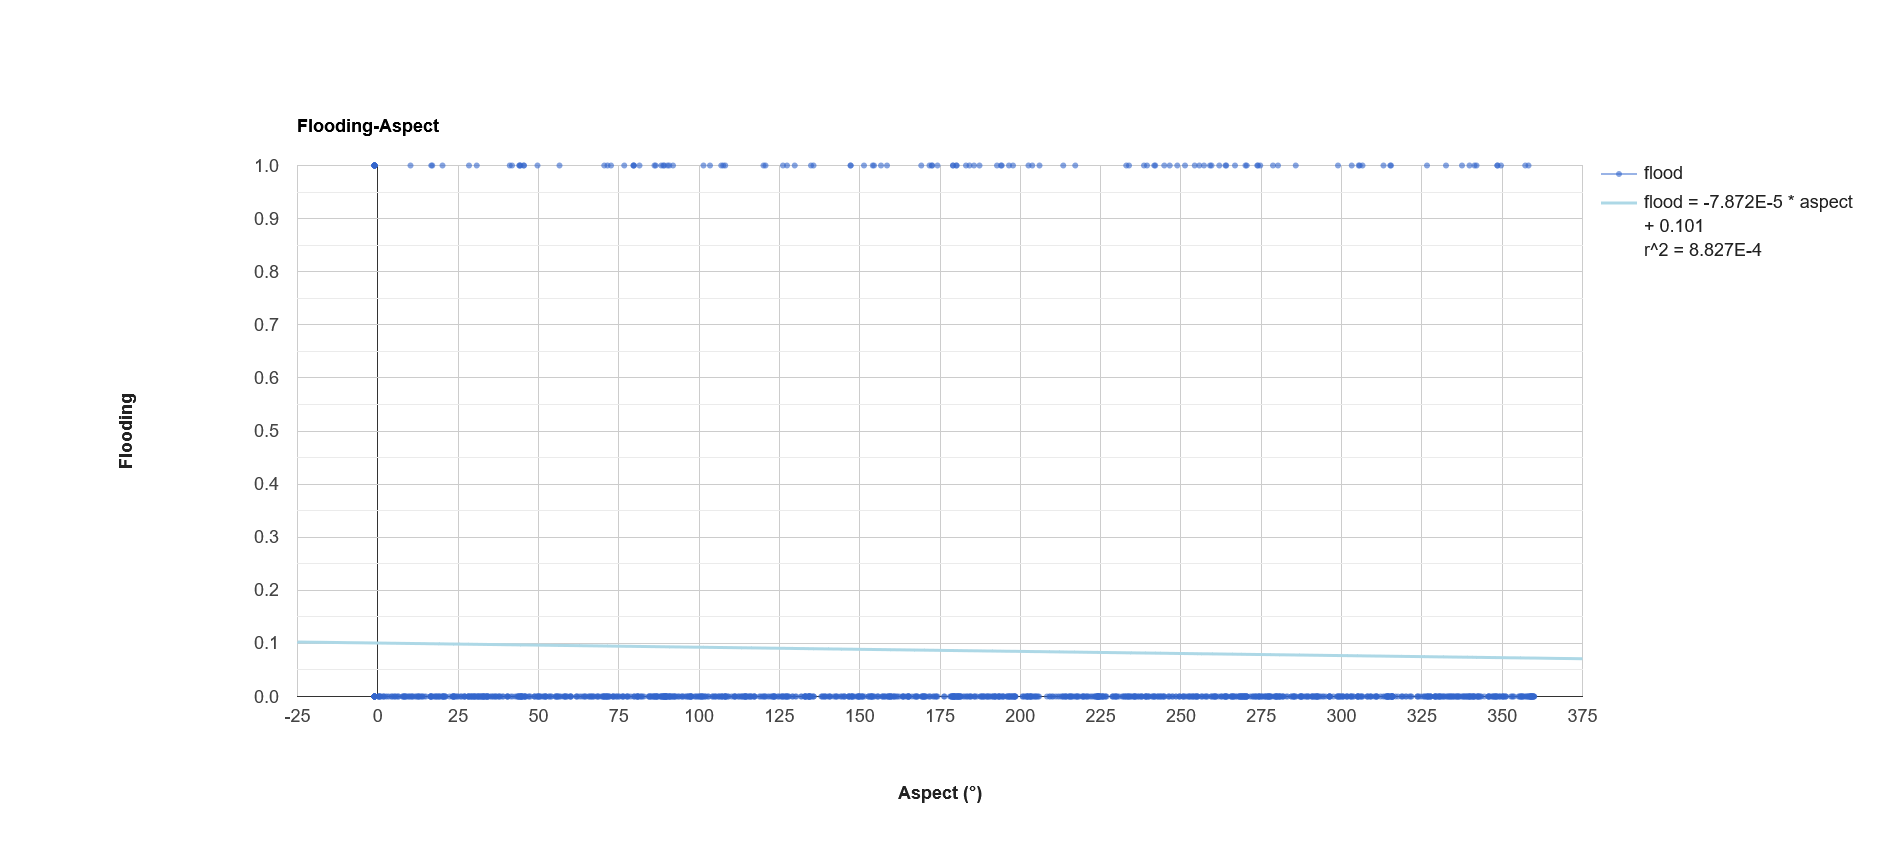
\includegraphics[keepaspectratio]{images/Collinearity/flood-aspect.png}}

}

\caption{\label{appfig-floodAspect}Linear regression analysis of flood
risk (binary) and aspect (°) for 5,000 randomly sampled points across
the full study area, encompassing Arizona.}

\end{appfig}%

\begin{appfig}

\centering{

\pandocbounded{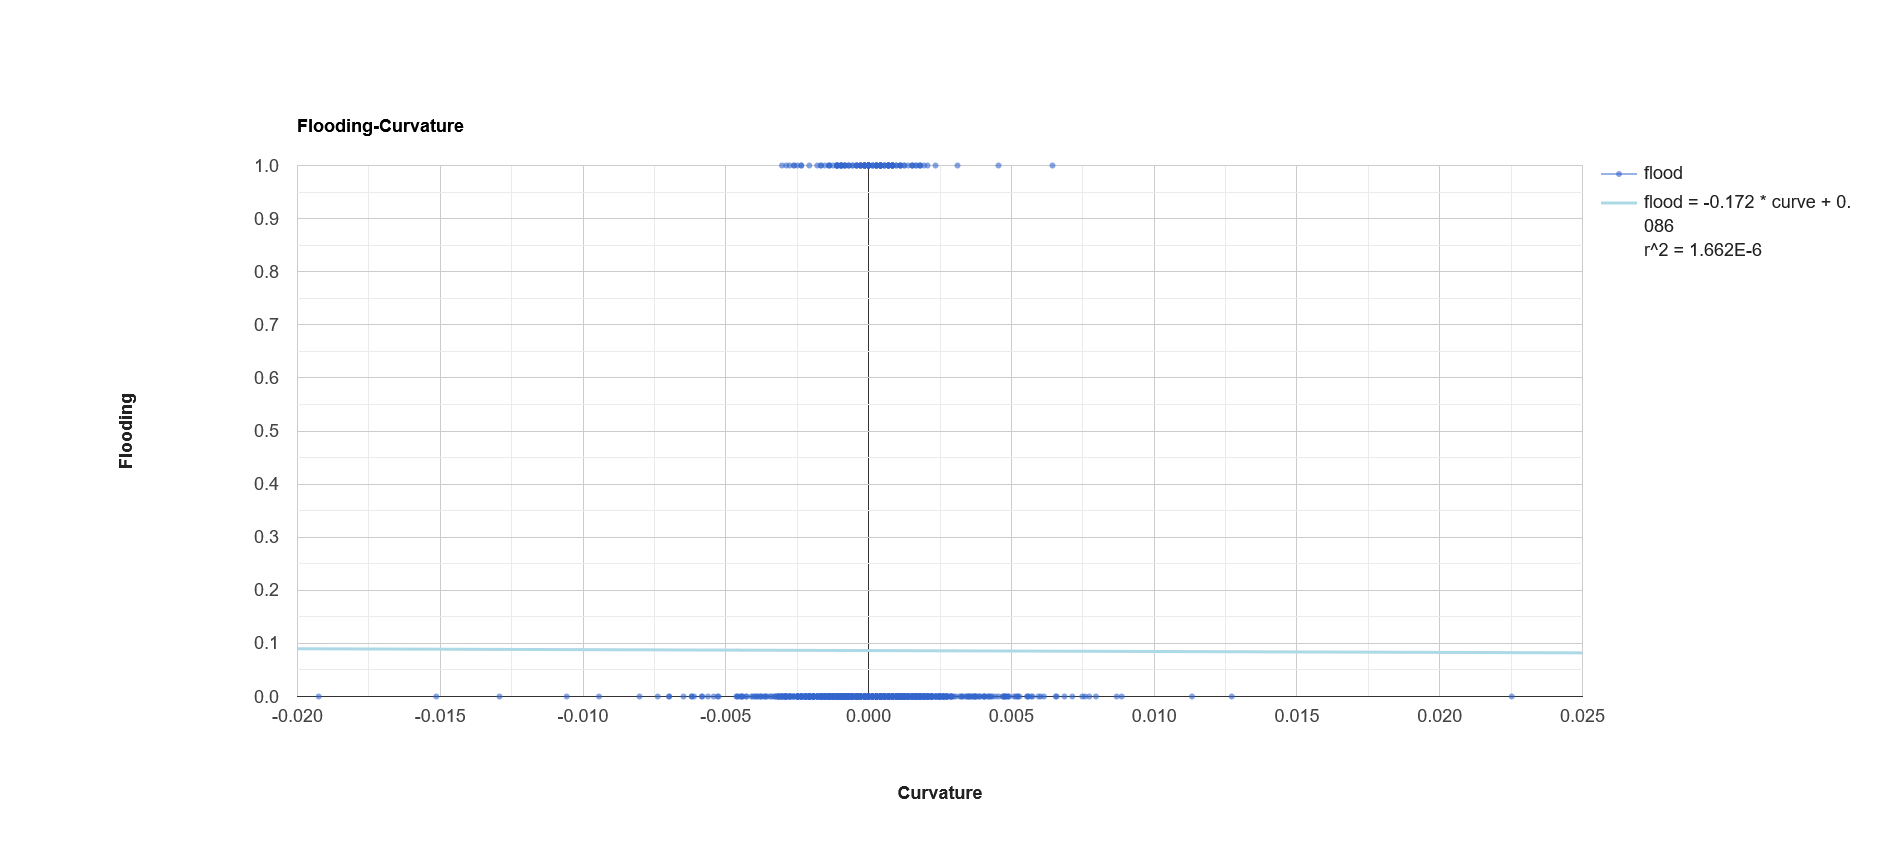
\includegraphics[keepaspectratio]{images/Collinearity/flood-curve.png}}

}

\caption{\label{appfig-floodCurve}Linear regression analysis of flood
risk (binary) and curvature for 5,000 randomly sampled points across the
full study area, encompassing Arizona.}

\end{appfig}%

\begin{appfig}

\centering{

\pandocbounded{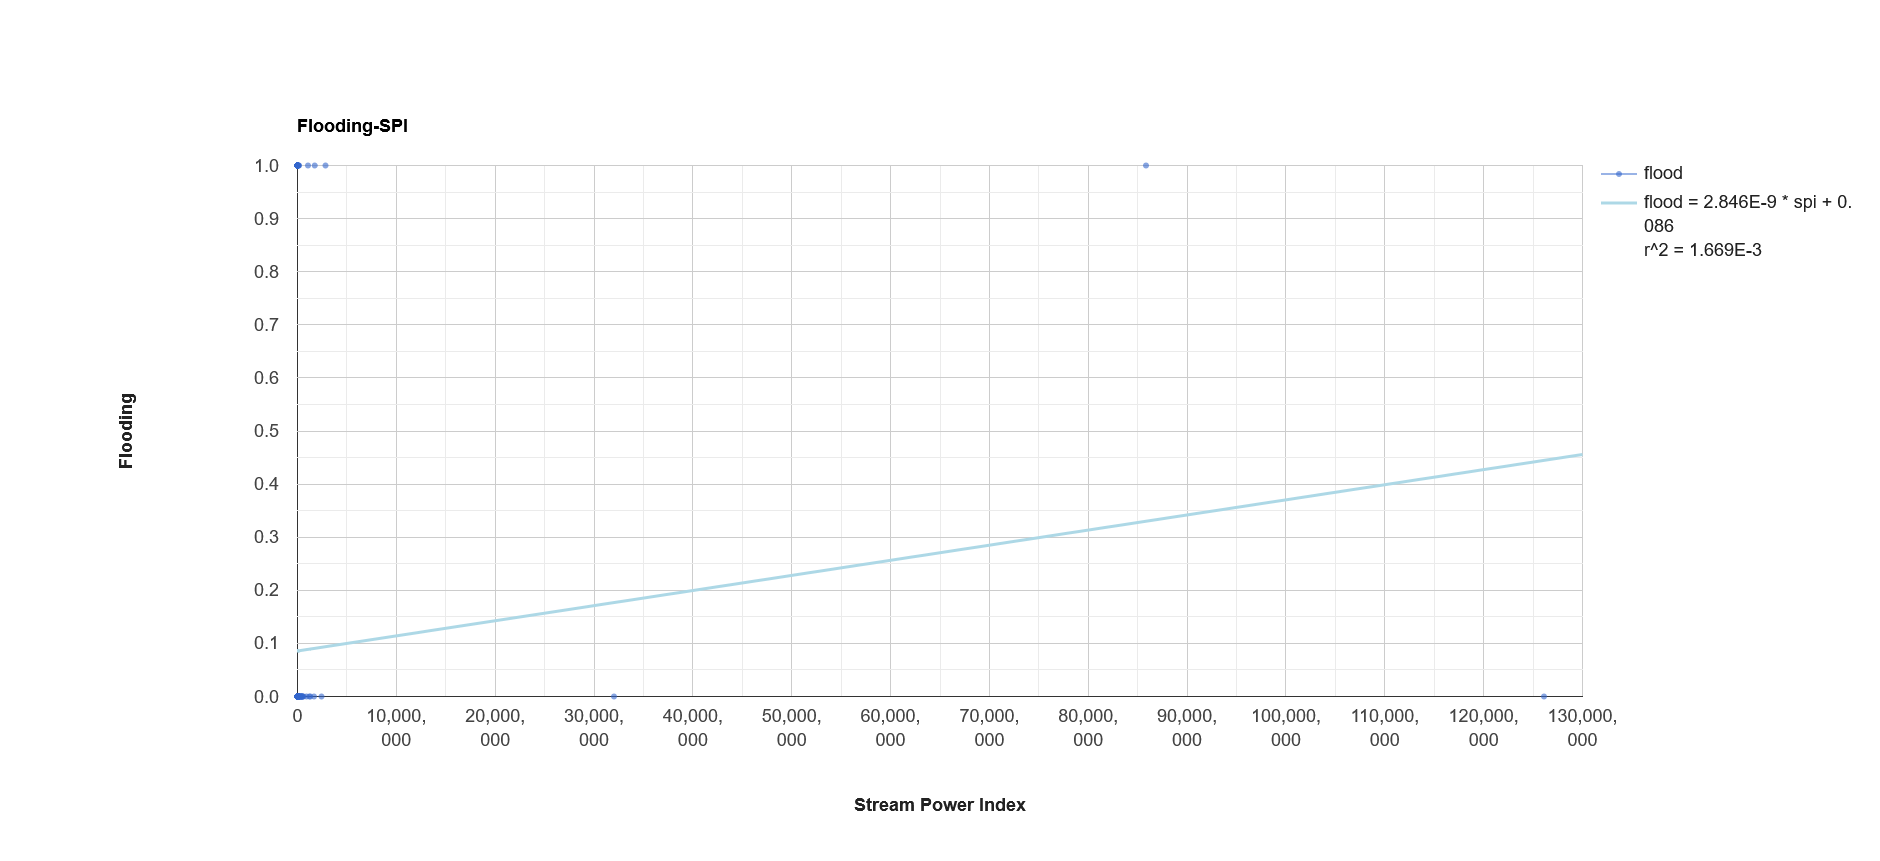
\includegraphics[keepaspectratio]{images/Collinearity/flood-spi.png}}

}

\caption{\label{appfig-floodSpi}Linear regression analysis of flood risk
(binary) and stream power index (SPI) for 5,000 randomly sampled points
across the full study area, encompassing Arizona.}

\end{appfig}%

\begin{appfig}

\centering{

\pandocbounded{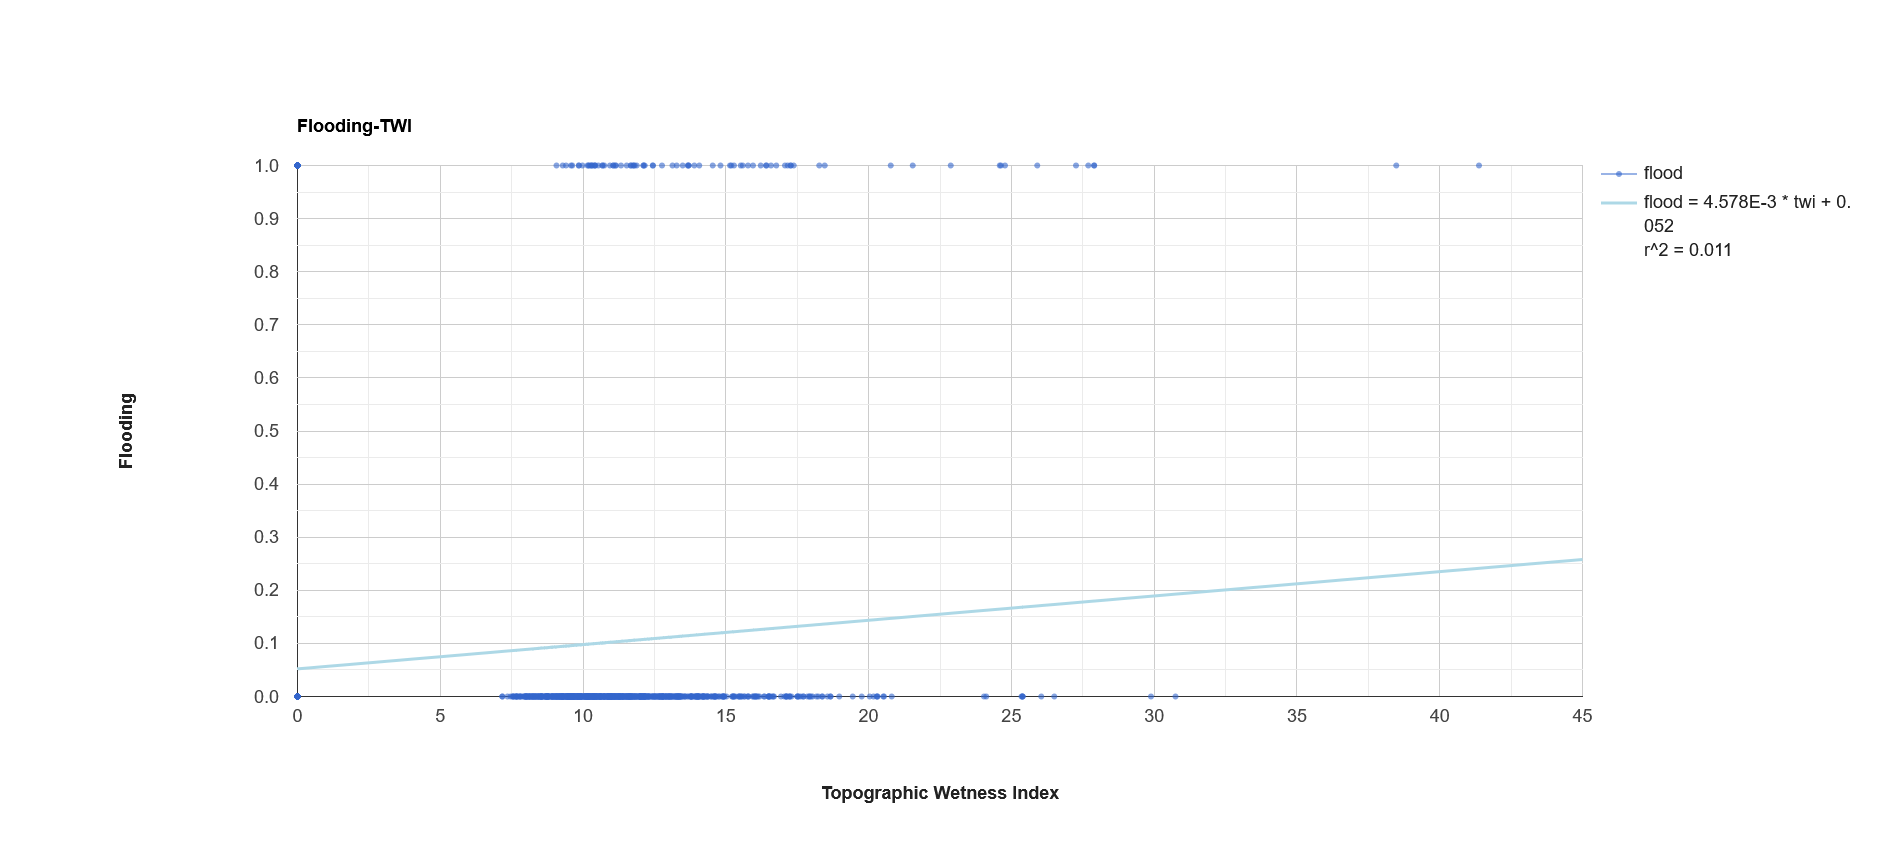
\includegraphics[keepaspectratio]{images/Collinearity/flood-twi.png}}

}

\caption{\label{appfig-floodTwi}Linear regression analysis of flood risk
(binary) and topographic wetness index (TWI) for 5,000 randomly sampled
points across the full study area, encompassing Arizona.}

\end{appfig}%

\begin{appfig}

\centering{

\pandocbounded{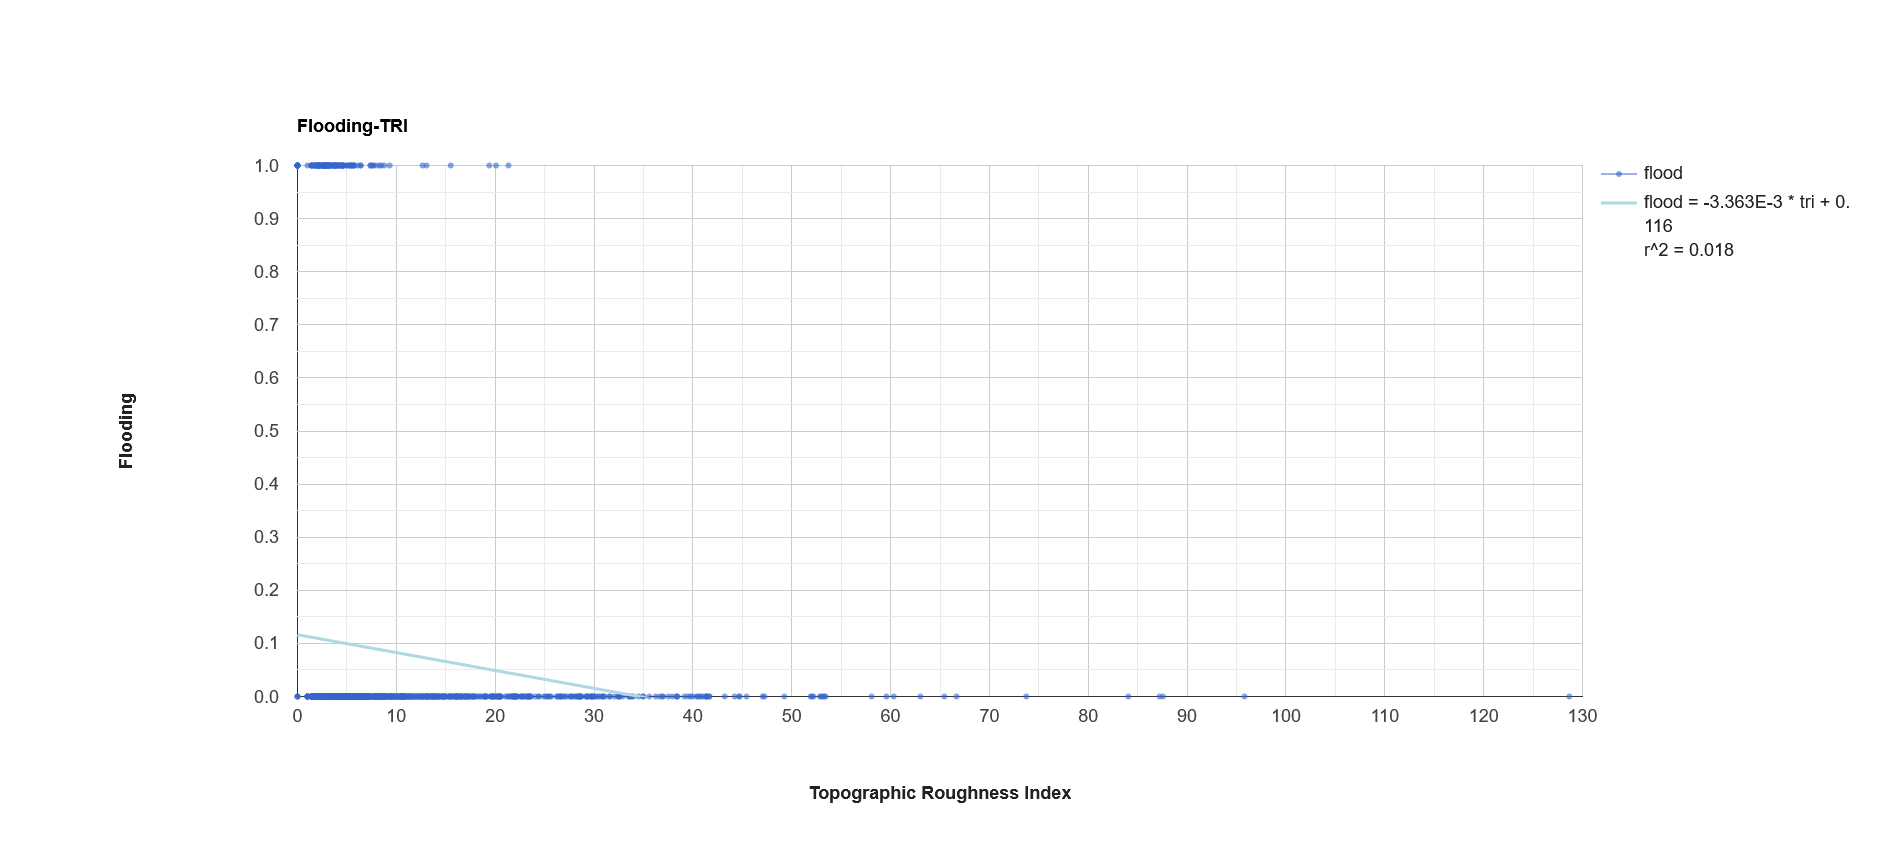
\includegraphics[keepaspectratio]{images/Collinearity/flood-tri.png}}

}

\caption{\label{appfig-floodTri}Linear regression analysis of flood risk
(binary) and topographic roughness index (TRI) for 5,000 randomly
sampled points across the full study area, encompassing Arizona.}

\end{appfig}%

\begin{appfig}

\centering{

\pandocbounded{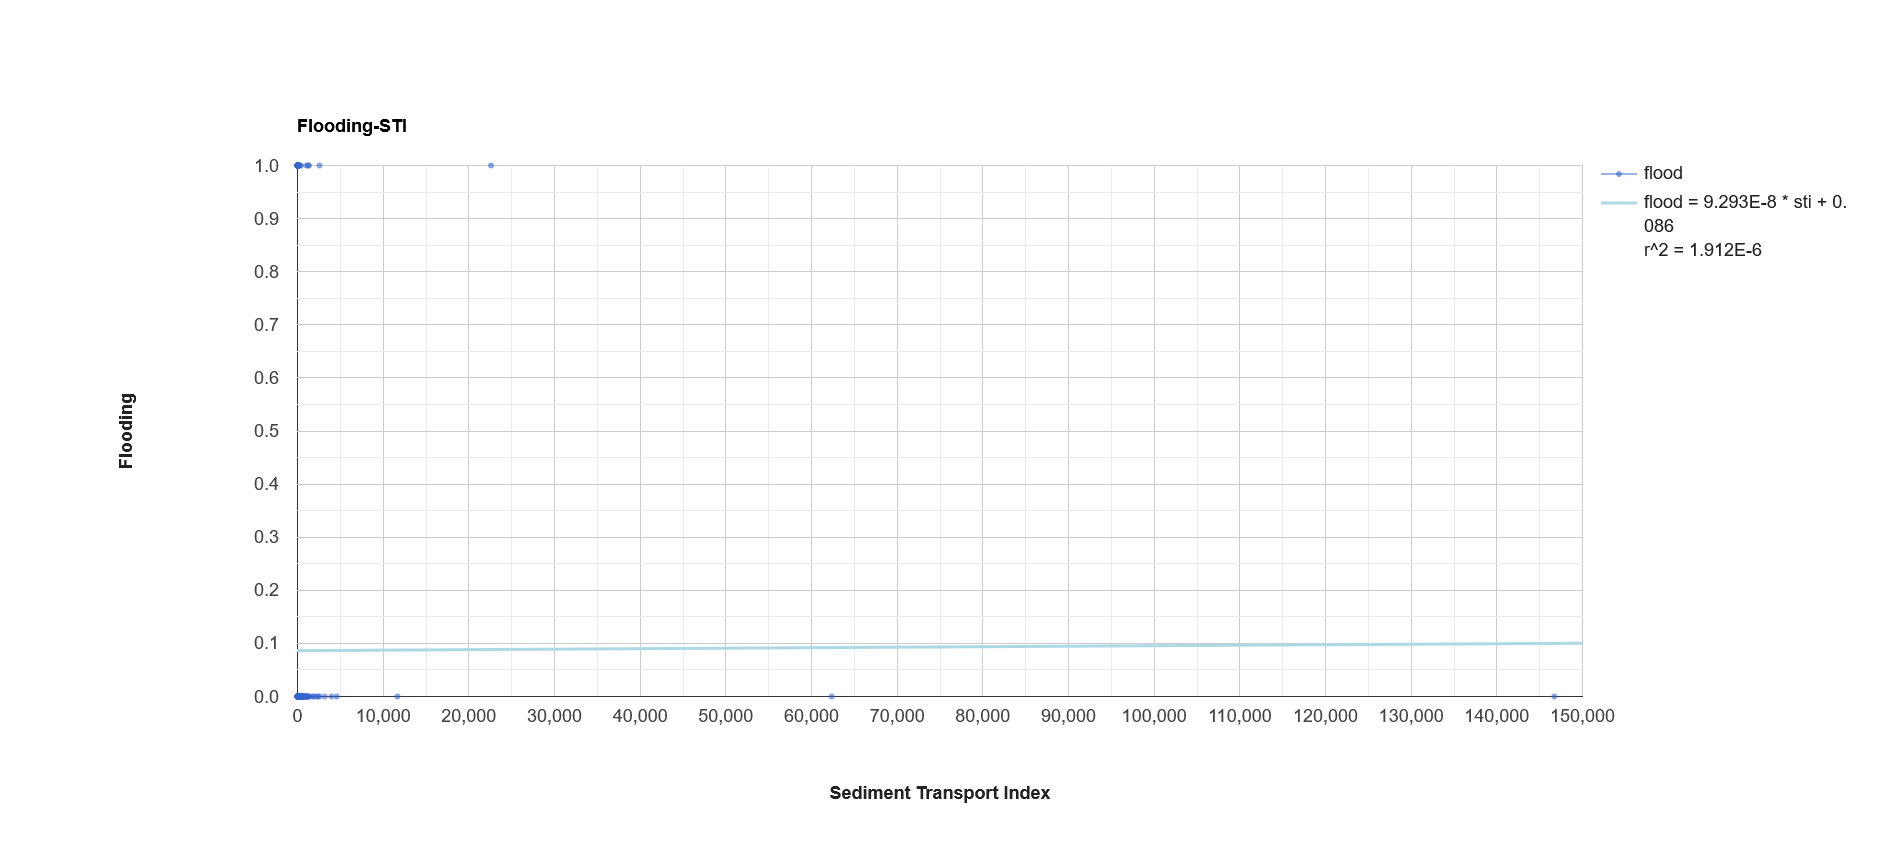
\includegraphics[keepaspectratio]{images/Collinearity/flood-sti.png}}

}

\caption{\label{appfig-floodSti}Linear regression analysis of flood risk
(binary) and sediment transport index (STI) for 5,000 randomly sampled
points across the full study area, encompassing Arizona.}

\end{appfig}%

\textbf{Elevation}

\begin{appfig}

\centering{

\pandocbounded{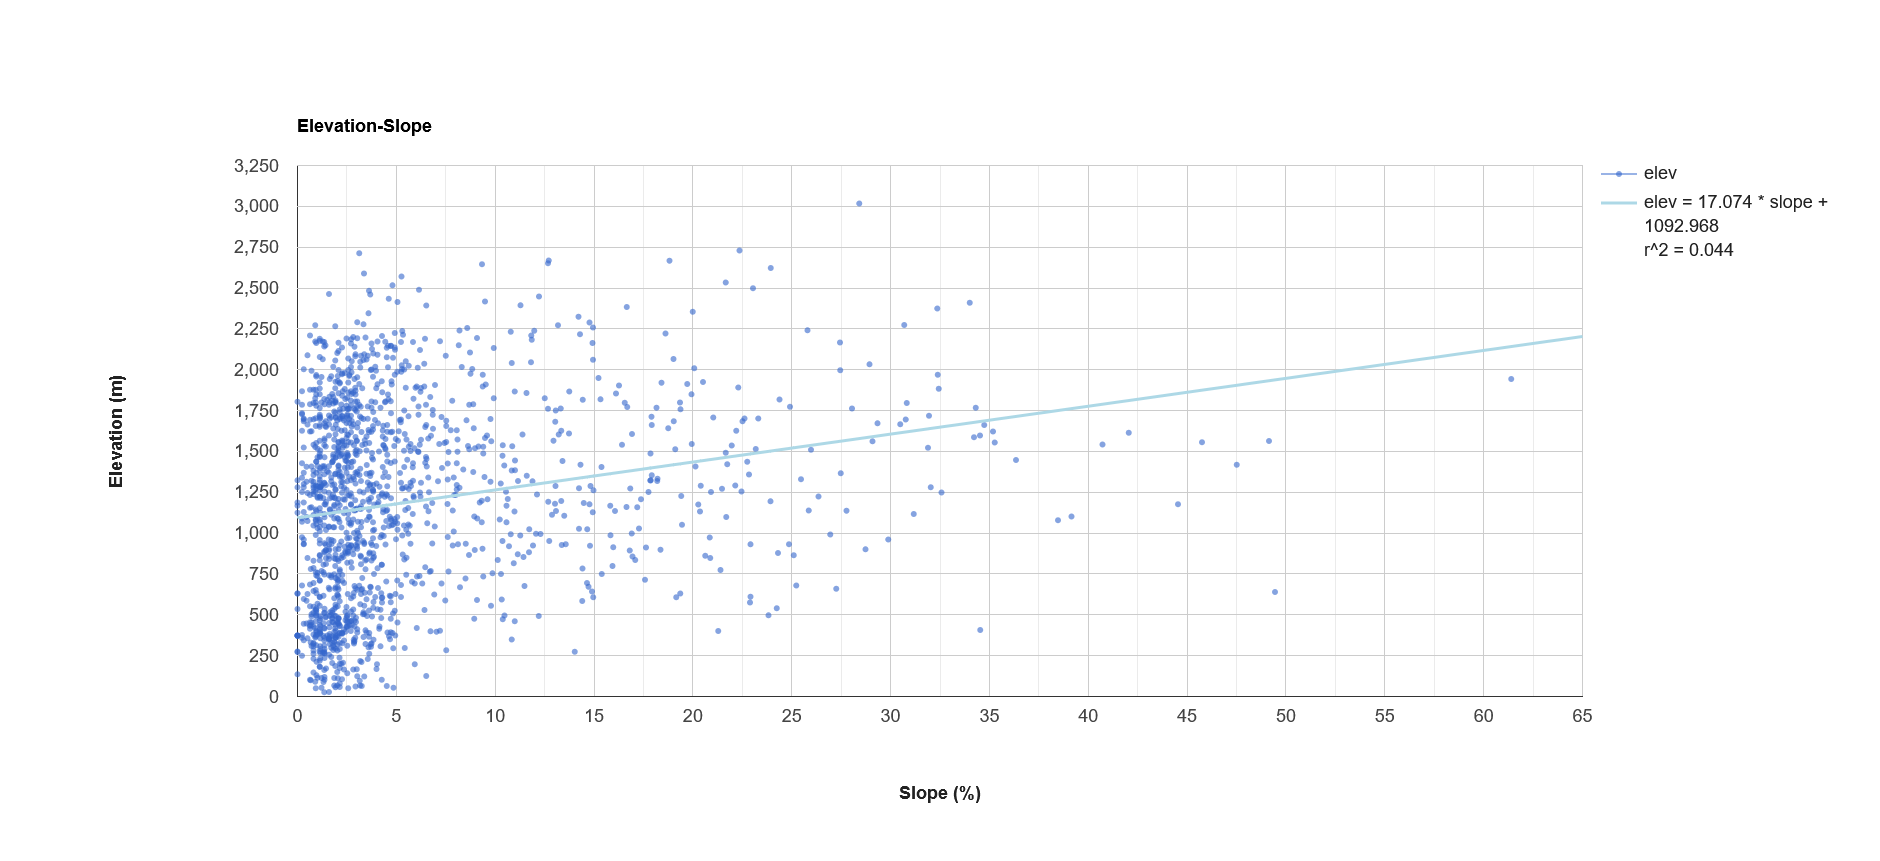
\includegraphics[keepaspectratio]{images/Collinearity/elev-slope.png}}

}

\caption{\label{appfig-elevSlope}Linear regression analysis of elevation
(m) and slope (°) for 5,000 randomly sampled points across the full
study area, encompassing Arizona.}

\end{appfig}%

\begin{appfig}

\centering{

\pandocbounded{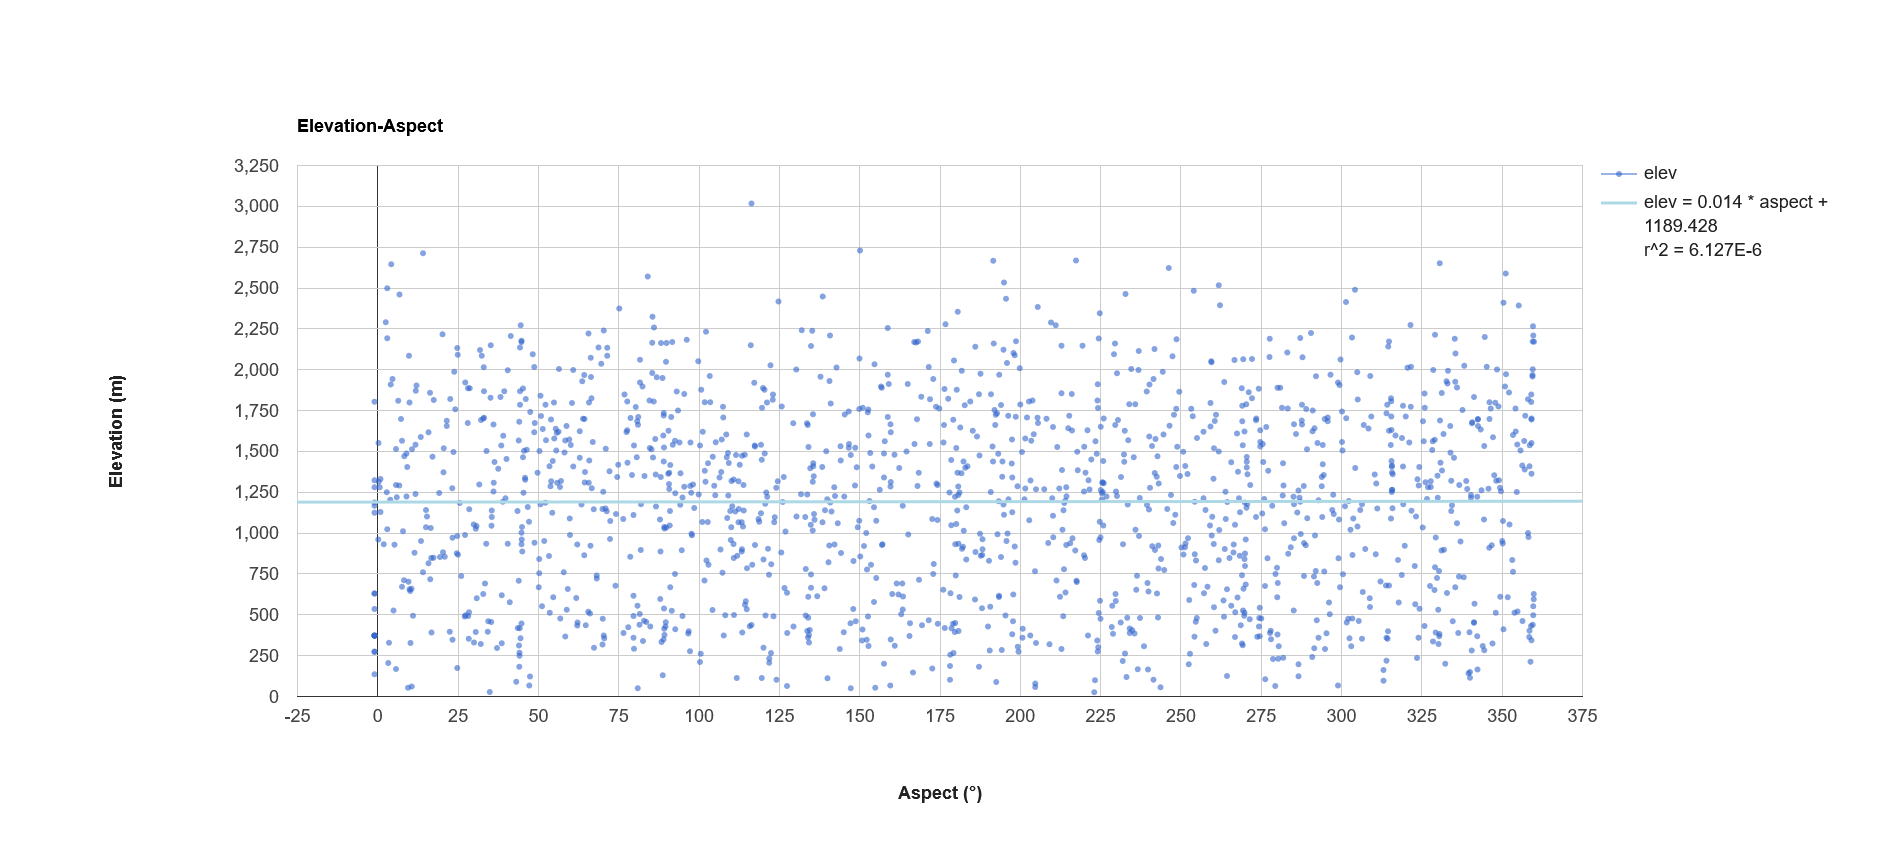
\includegraphics[keepaspectratio]{images/Collinearity/elev-aspect.png}}

}

\caption{\label{appfig-elevAspect}Linear regression analysis of
elevation (m) and aspect (°) for 5,000 randomly sampled points across
the full study area, encompassing Arizona.}

\end{appfig}%

\begin{appfig}

\centering{

\pandocbounded{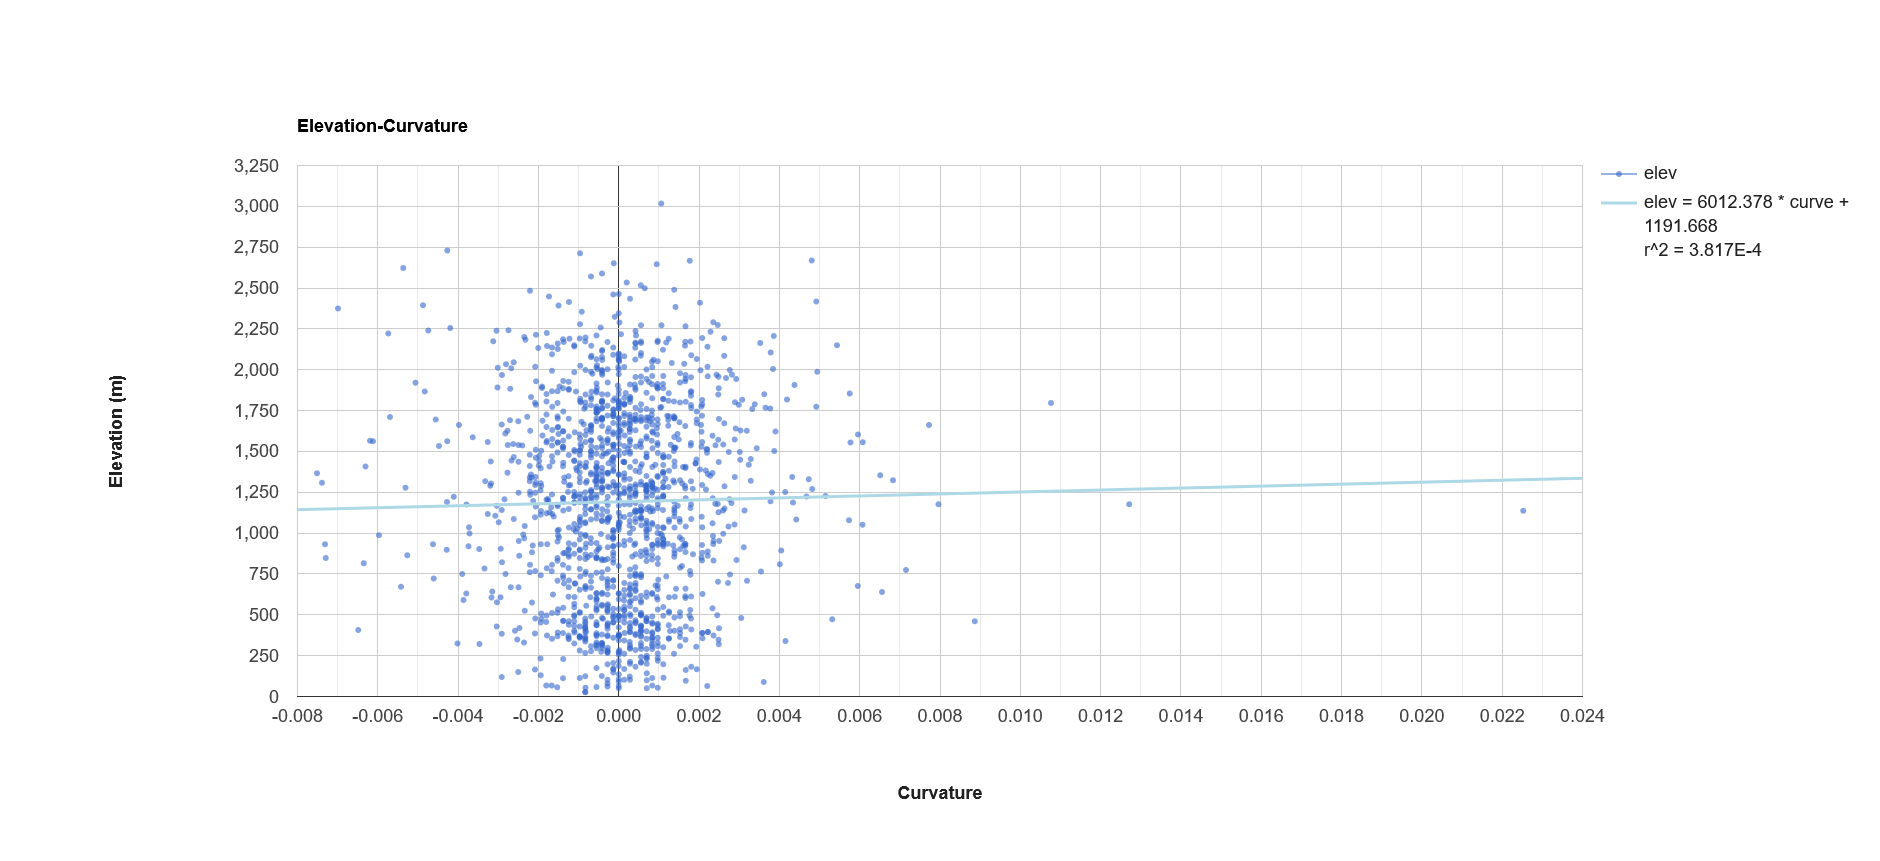
\includegraphics[keepaspectratio]{images/Collinearity/elev-curve.png}}

}

\caption{\label{appfig-elevCurve}Linear regression analysis of elevation
(m) and curvature for 5,000 randomly sampled points across the full
study area, encompassing Arizona.}

\end{appfig}%

\begin{appfig}

\centering{

\pandocbounded{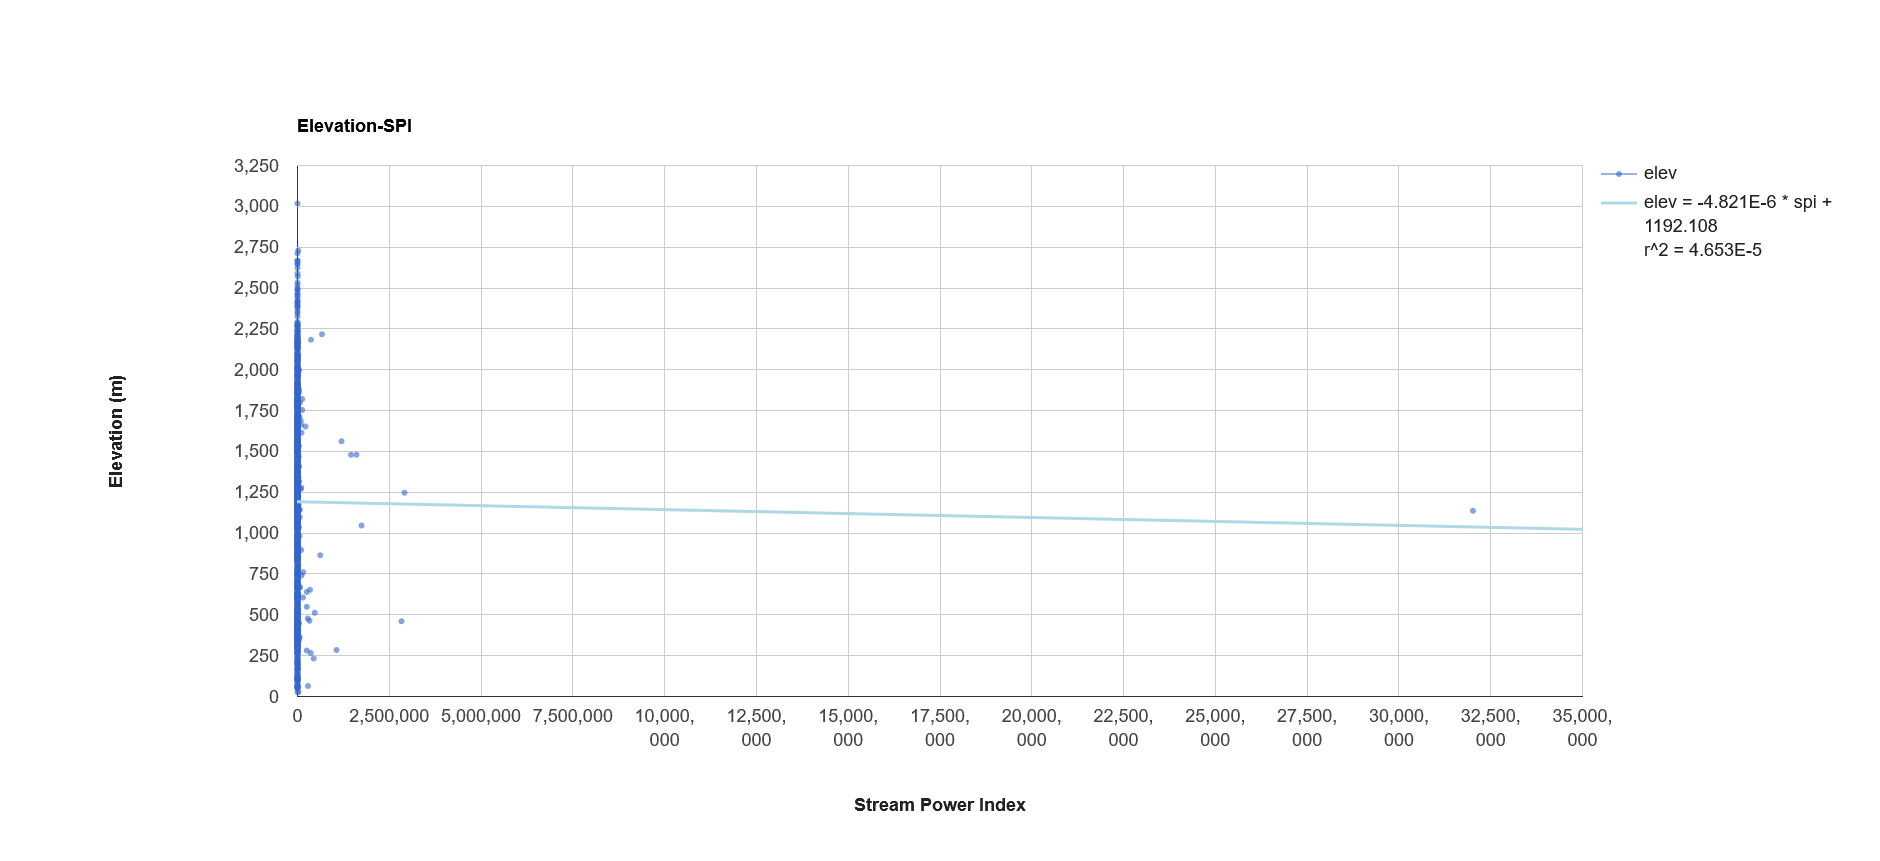
\includegraphics[keepaspectratio]{images/Collinearity/elev-spi.png}}

}

\caption{\label{appfig-elevSpi}Linear regression analysis of elevation
(m) and stream power index (SPI) for 5,000 randomly sampled points
across the full study area, encompassing Arizona.}

\end{appfig}%

\begin{appfig}

\centering{

\pandocbounded{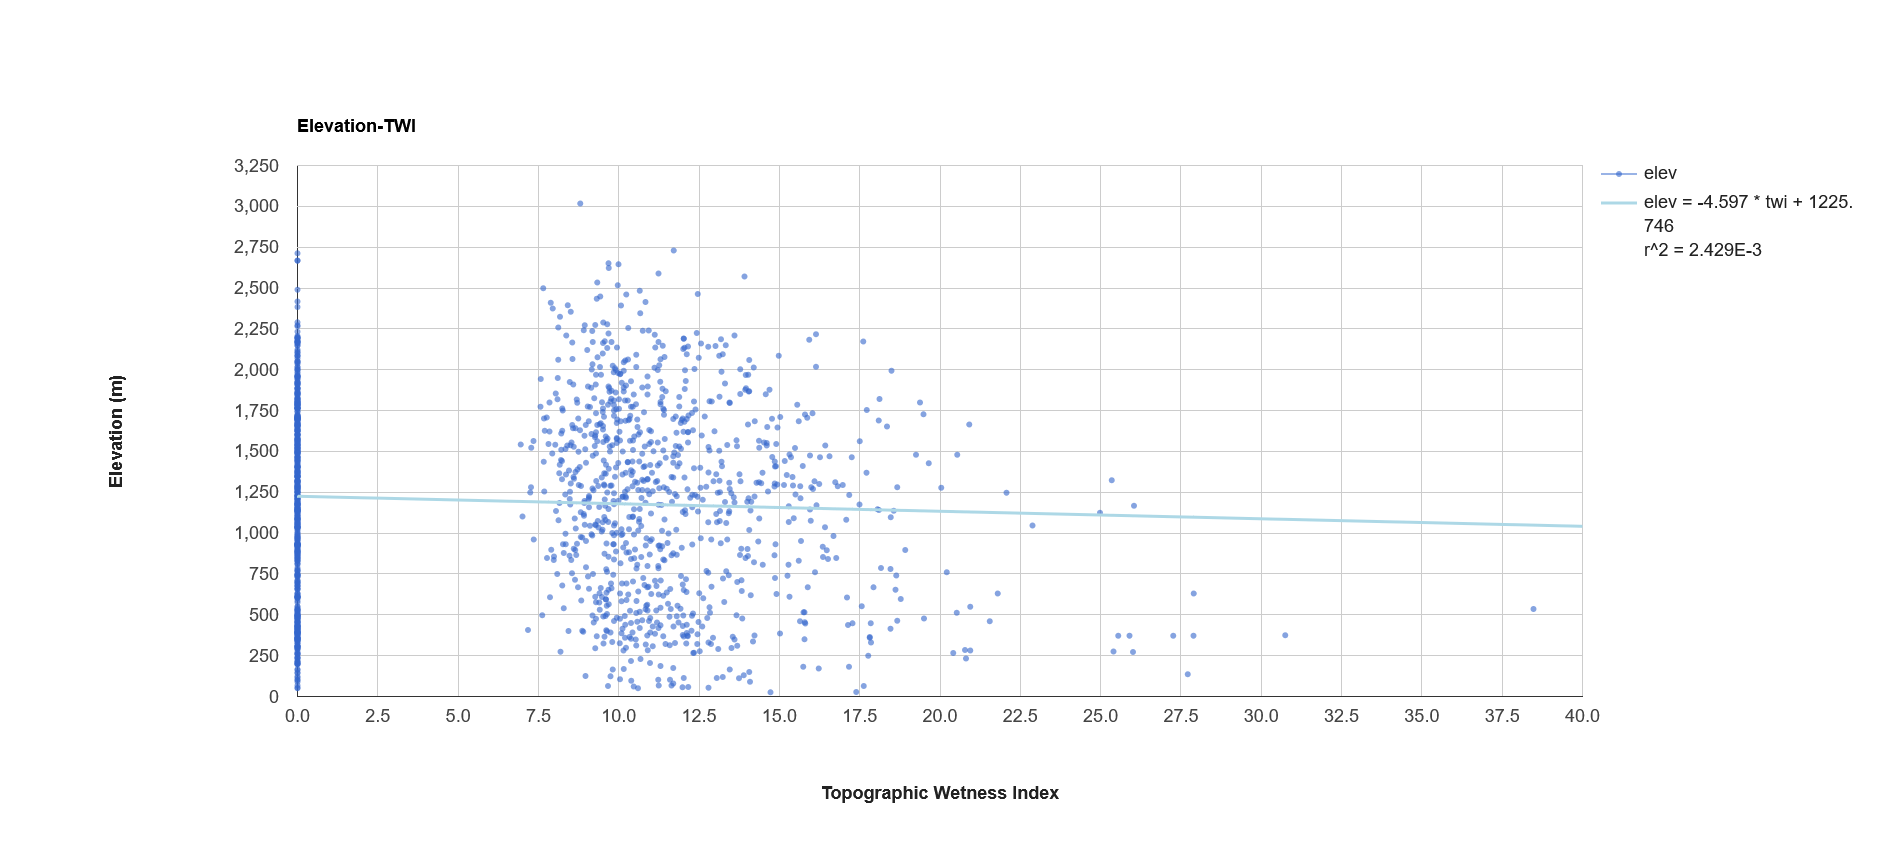
\includegraphics[keepaspectratio]{images/Collinearity/elev-twi.png}}

}

\caption{\label{appfig-elevTwi}Linear regression analysis of elevation
(m) and topographic wetness index (TWI) for 5,000 randomly sampled
points across the full study area, encompassing Arizona.}

\end{appfig}%

\begin{appfig}

\centering{

\pandocbounded{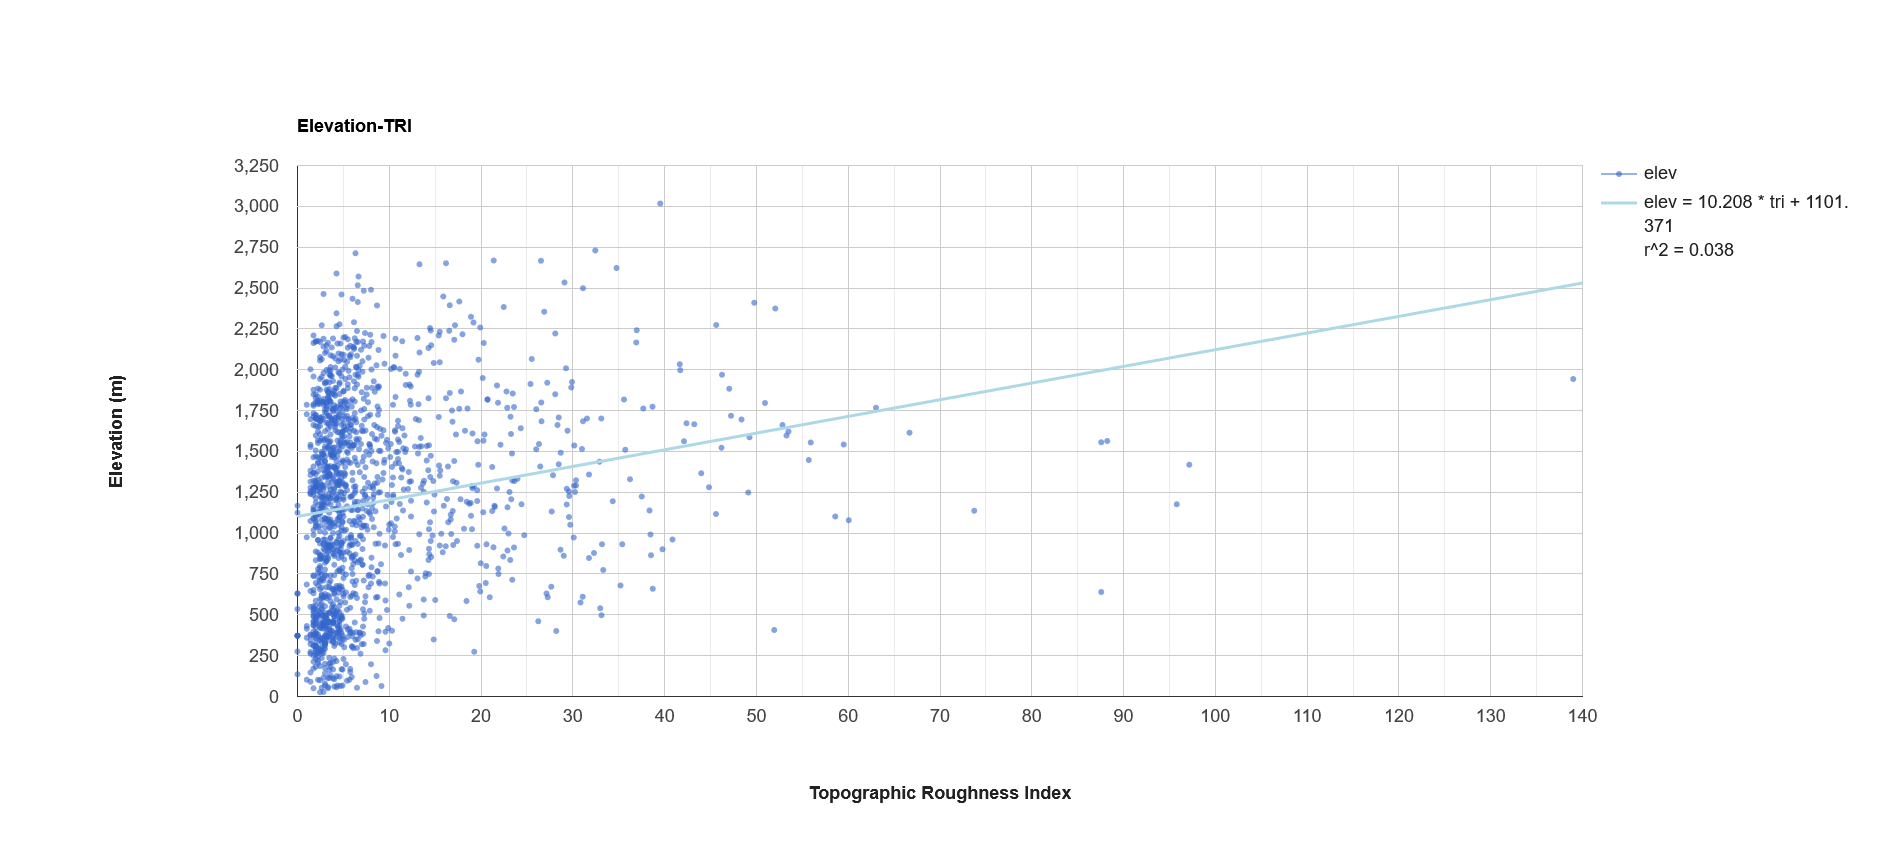
\includegraphics[keepaspectratio]{images/Collinearity/elev-tri.png}}

}

\caption{\label{appfig-elevTri}Linear regression analysis of elevation
(m) and topographic roughness index (TRI) for 5,000 randomly sampled
points across the full study area, encompassing Arizona.}

\end{appfig}%

\begin{appfig}

\centering{

\pandocbounded{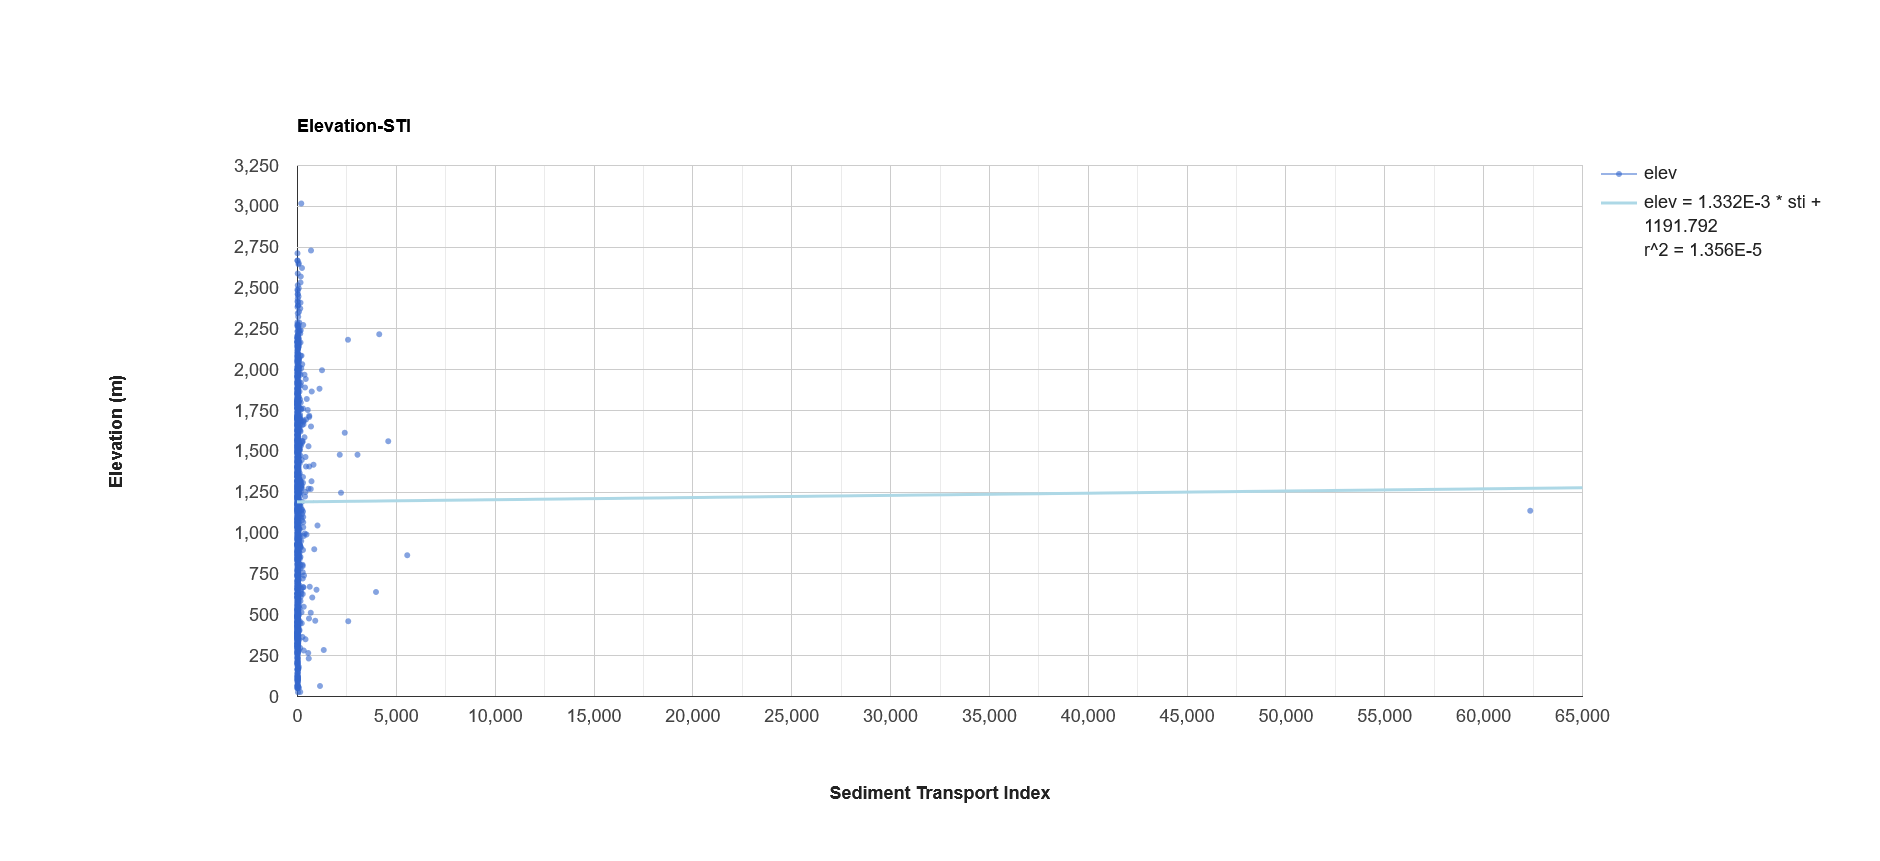
\includegraphics[keepaspectratio]{images/Collinearity/elev-sti.png}}

}

\caption{\label{appfig-elevSti}Linear regression analysis of elevation
(m) and sediment transport index (STI) for 5,000 randomly sampled points
across the full study area, encompassing Arizona.}

\end{appfig}%

\textbf{Slope}

\begin{appfig}

\centering{

\pandocbounded{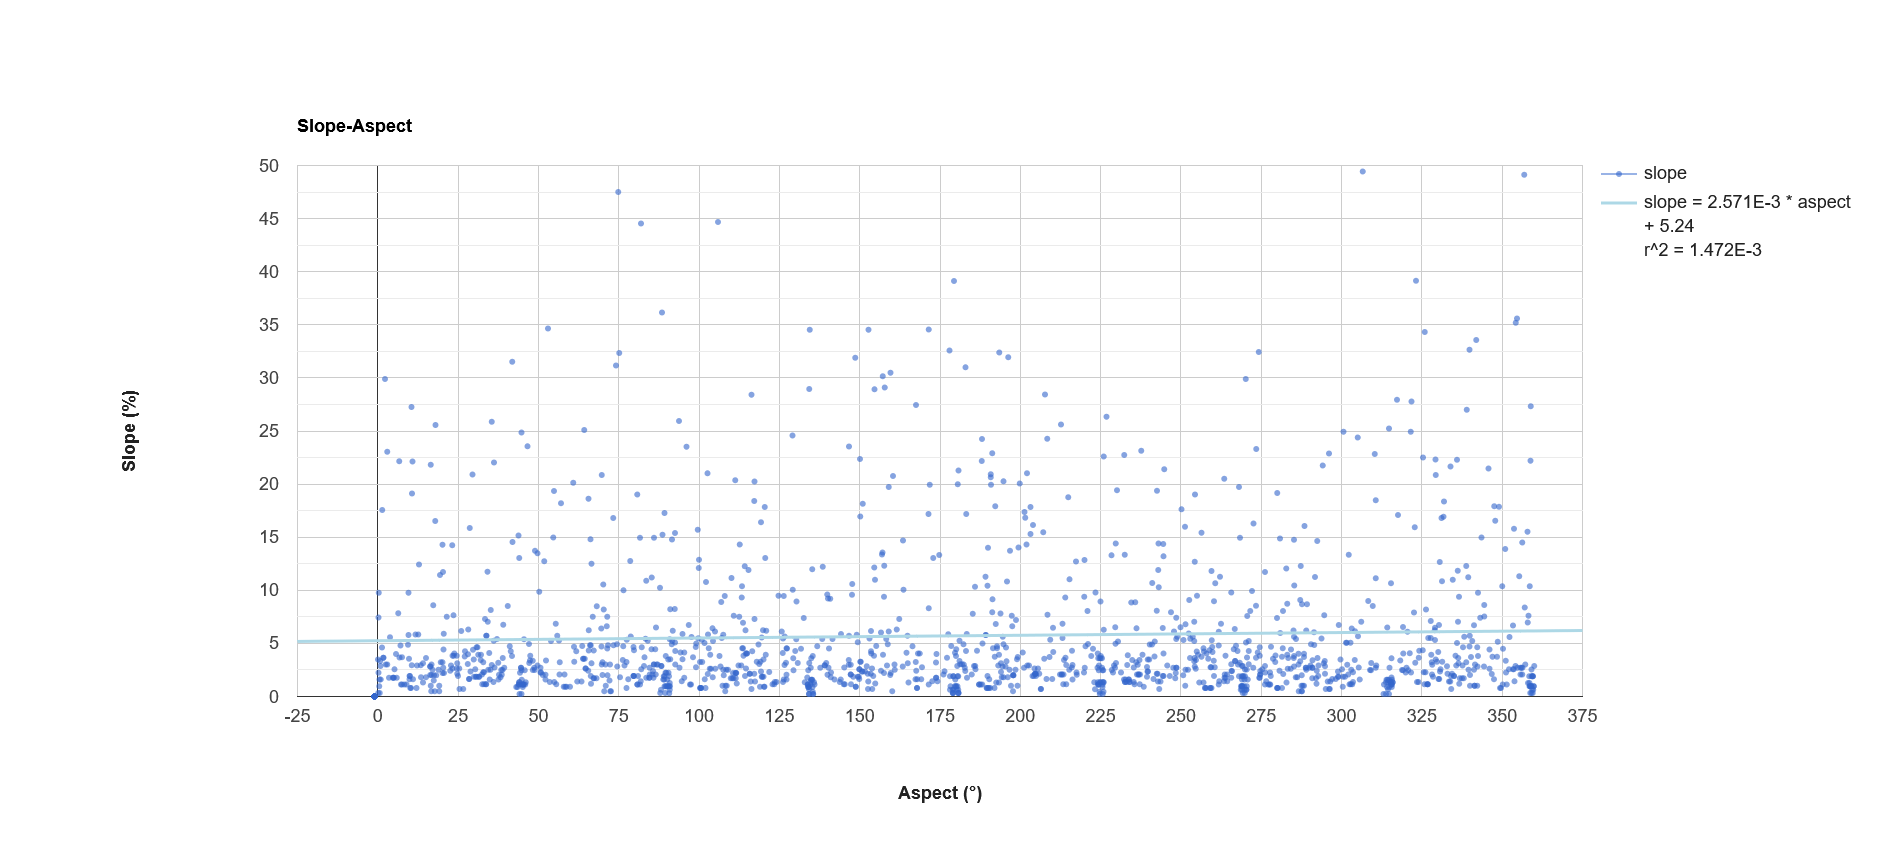
\includegraphics[keepaspectratio]{images/Collinearity/slope-aspect.png}}

}

\caption{\label{appfig-slopeAspect}Linear regression analysis of slope
(°) and aspect (°) for 5,000 randomly sampled points across the full
study area, encompassing Arizona.}

\end{appfig}%

\begin{appfig}

\centering{

\pandocbounded{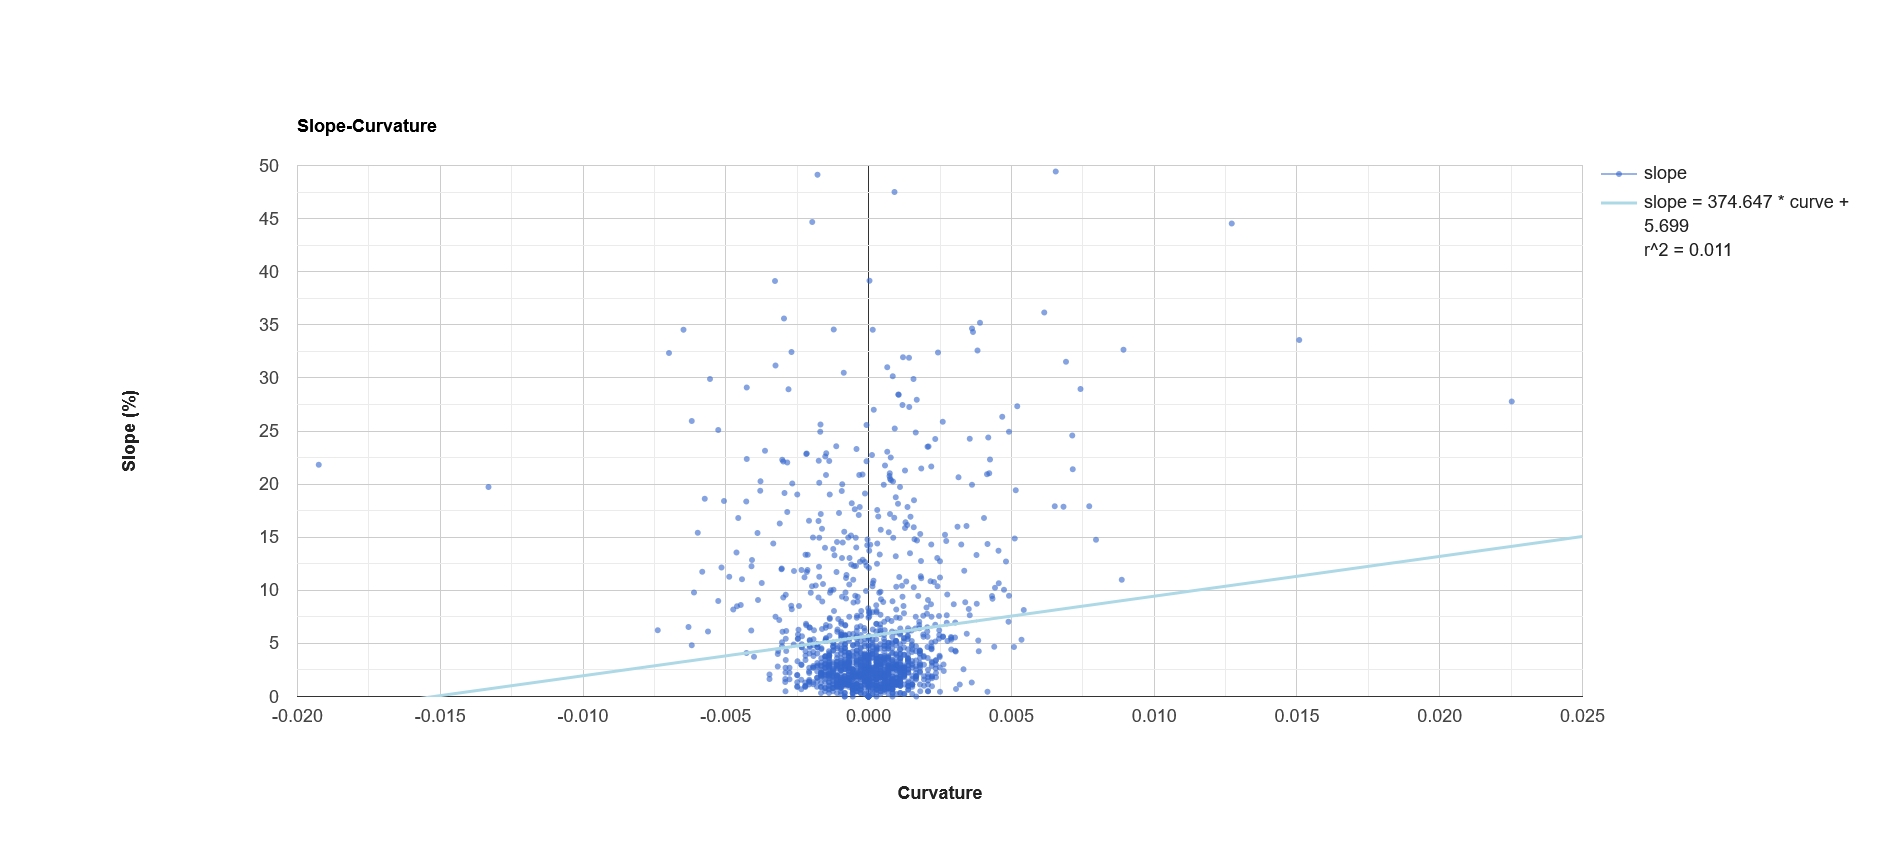
\includegraphics[keepaspectratio]{images/Collinearity/slope-curve.png}}

}

\caption{\label{appfig-slopeCurve}Linear regression analysis of slope
(°) and curvature for 5,000 randomly sampled points across the full
study area, encompassing Arizona.}

\end{appfig}%

\begin{appfig}

\centering{

\pandocbounded{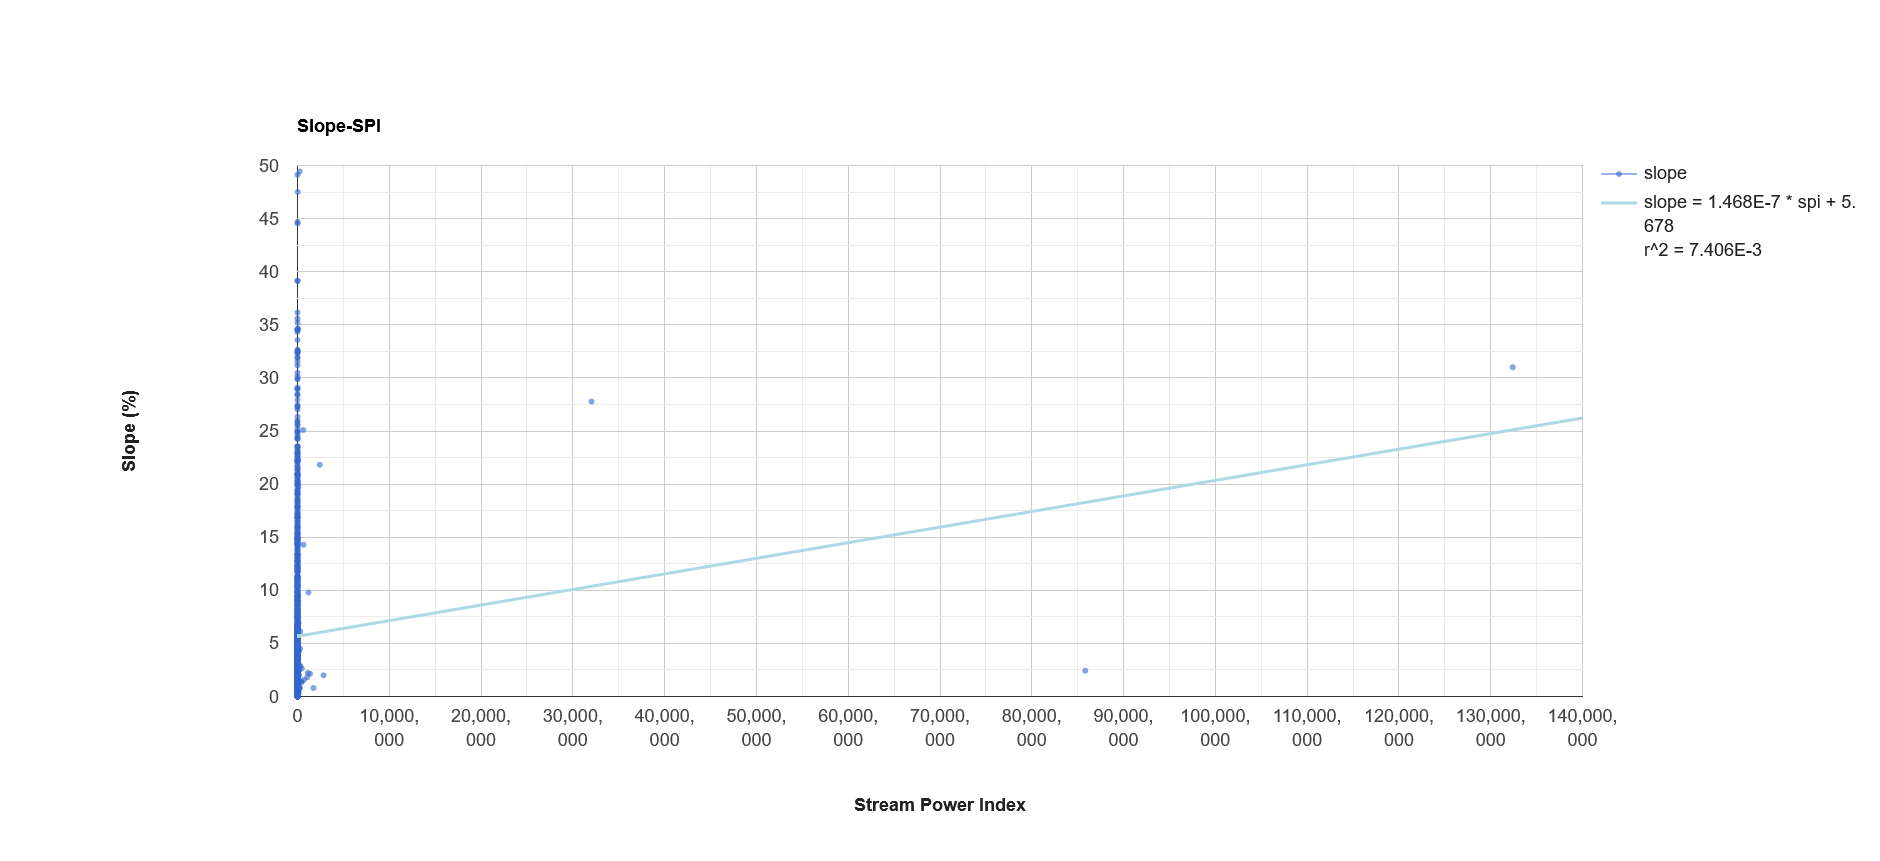
\includegraphics[keepaspectratio]{images/Collinearity/slope-spi.png}}

}

\caption{\label{appfig-slopeSpi}Linear regression analysis of slope (°)
and stream power index (SPI) for 5,000 randomly sampled points across
the full study area, encompassing Arizona.}

\end{appfig}%

\begin{appfig}

\centering{

\pandocbounded{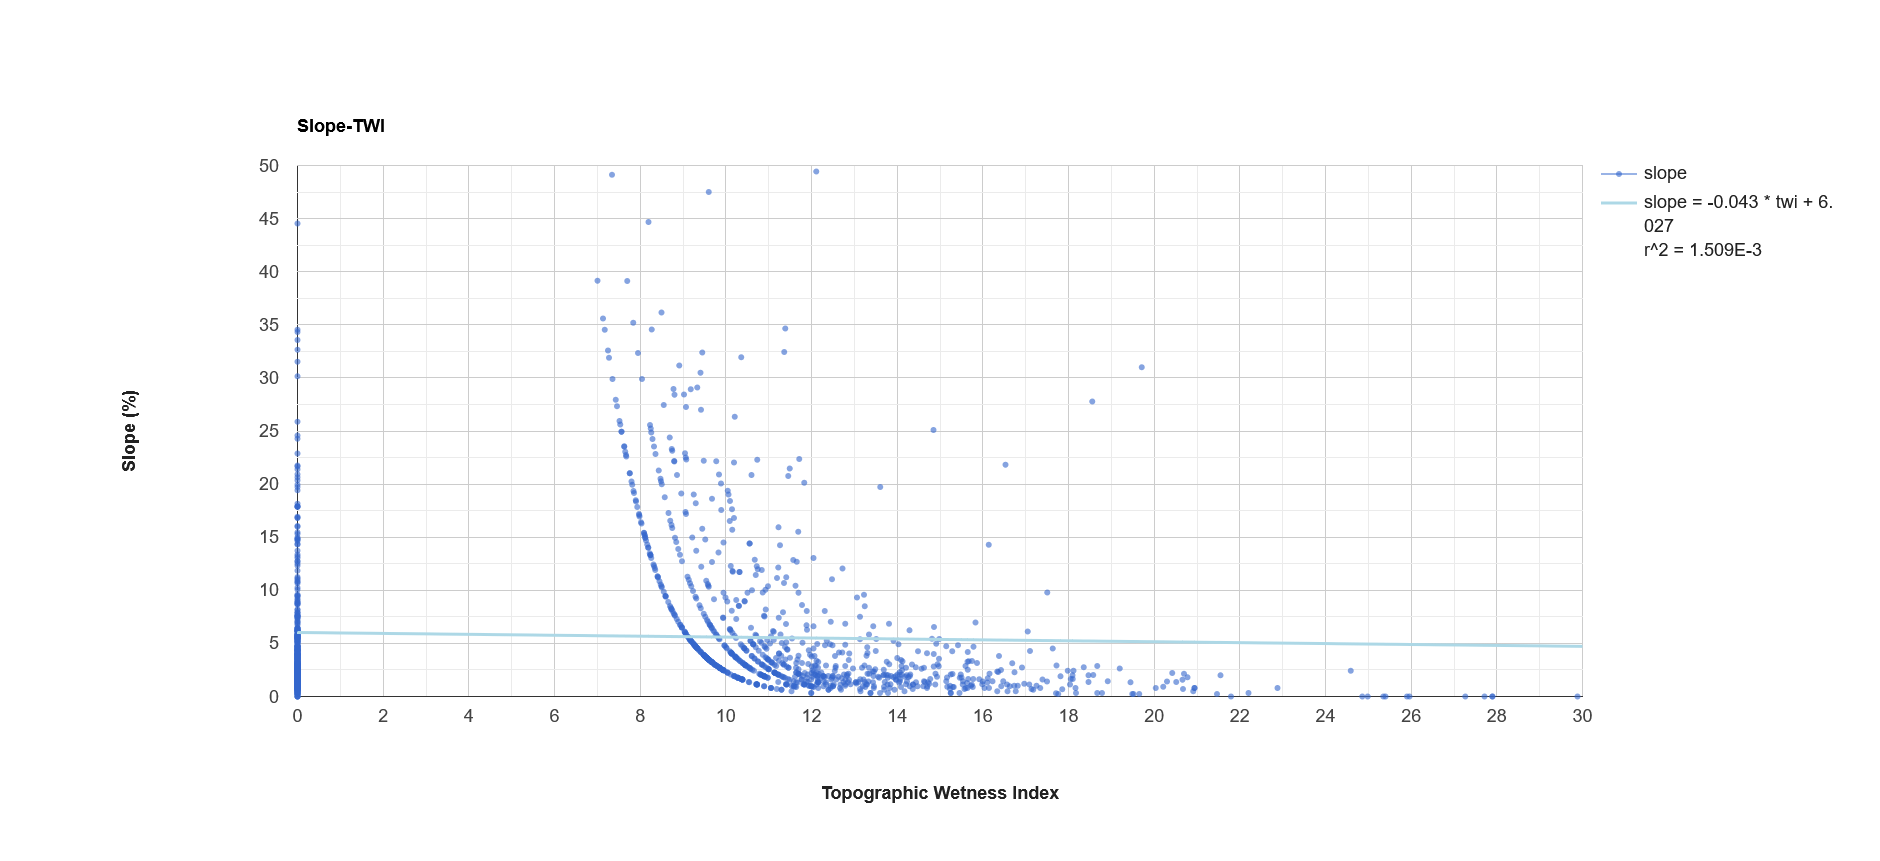
\includegraphics[keepaspectratio]{images/Collinearity/slope-twi.png}}

}

\caption{\label{appfig-slopeTwi}Linear regression analysis of slope (°)
and topographic wetness index (TWI) for 5,000 randomly sampled points
across the full study area, encompassing Arizona.}

\end{appfig}%

\begin{appfig}

\centering{

\pandocbounded{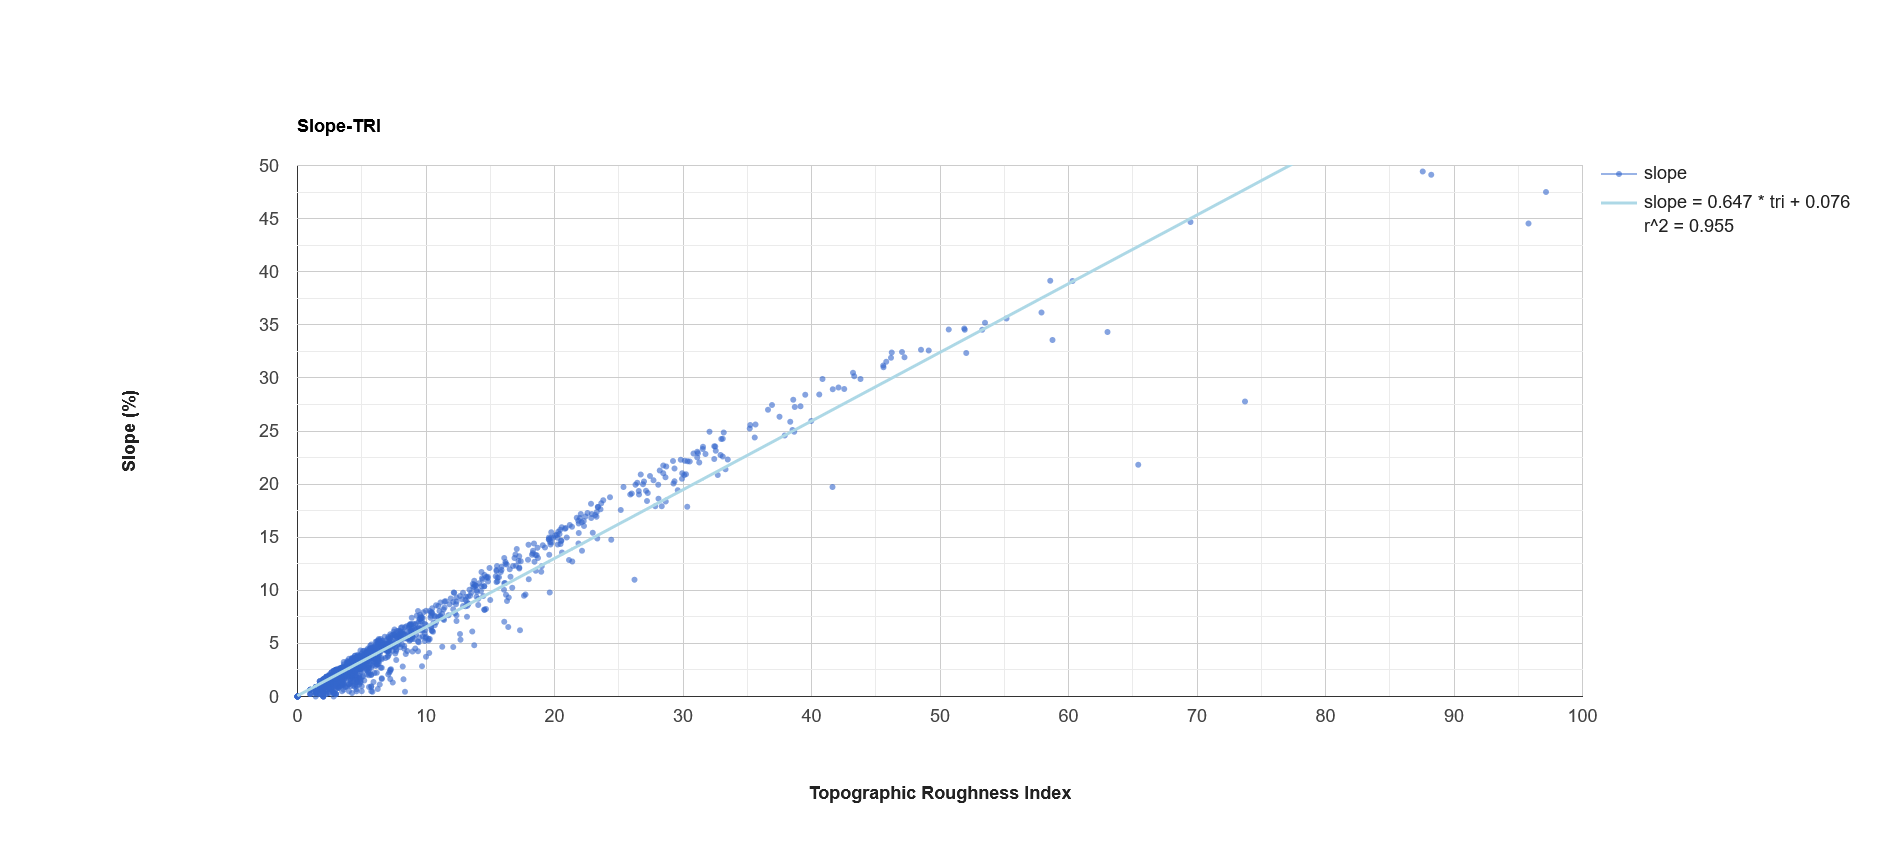
\includegraphics[keepaspectratio]{images/Collinearity/slope-tri.png}}

}

\caption{\label{appfig-slopeTri}Linear regression analysis of slope (°)
and topographic roughness index (TRI) for 5,000 randomly sampled points
across the full study area, encompassing Arizona.}

\end{appfig}%

\begin{appfig}

\centering{

\pandocbounded{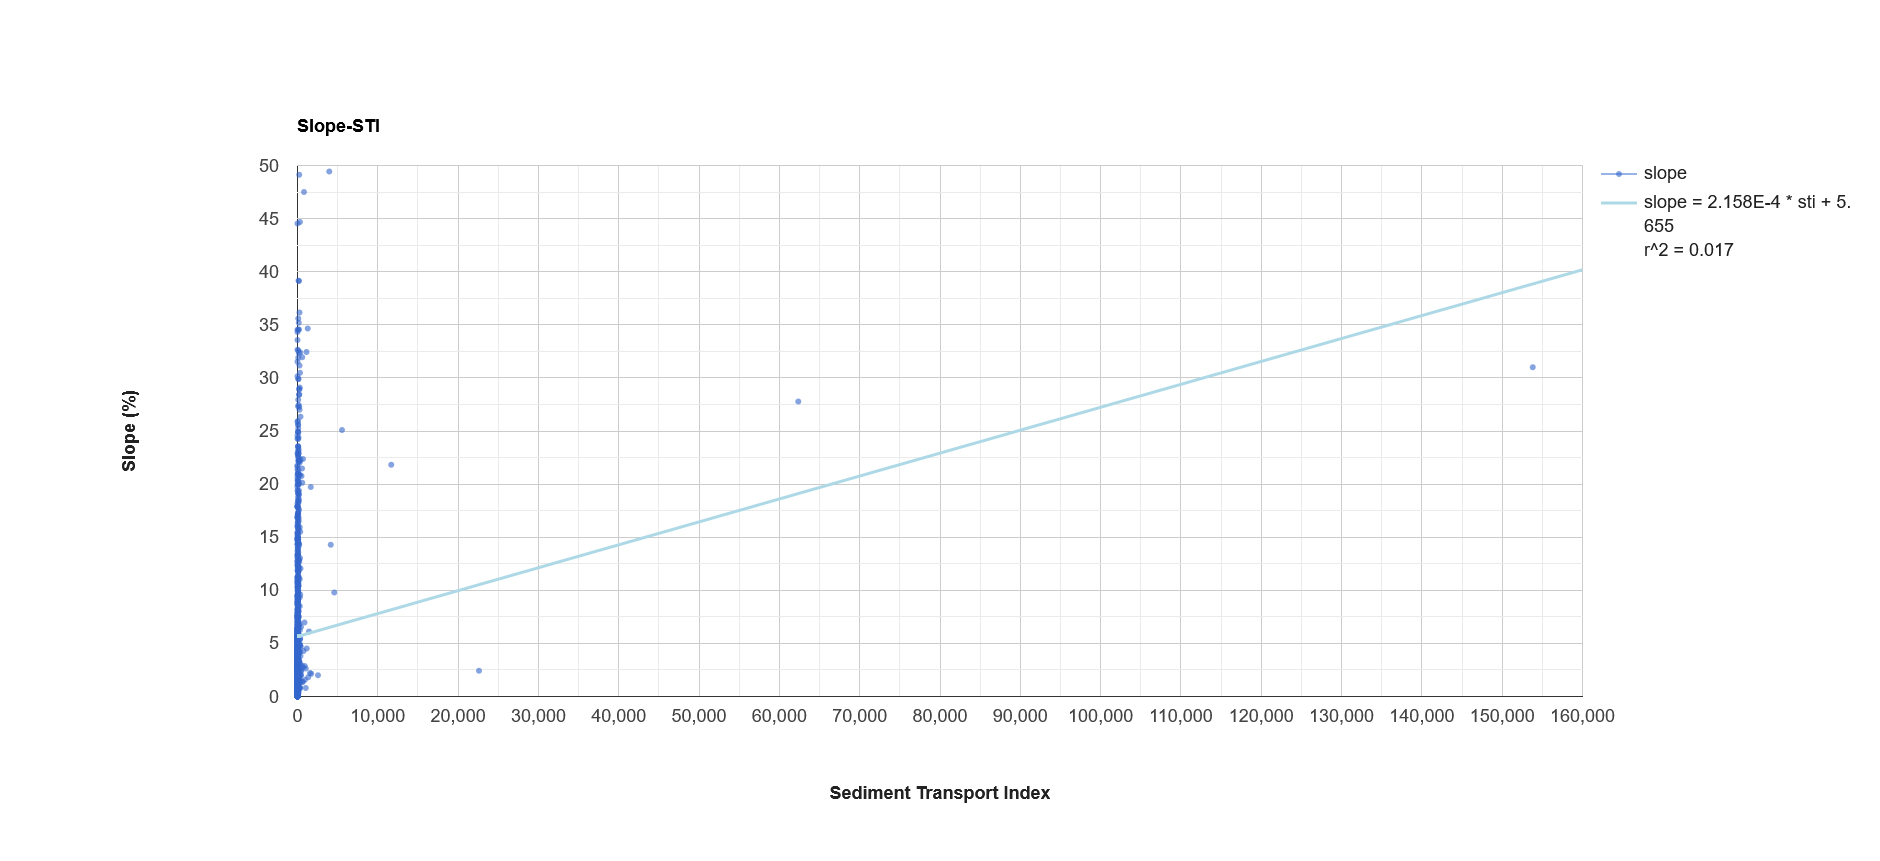
\includegraphics[keepaspectratio]{images/Collinearity/slope-sti.png}}

}

\caption{\label{appfig-slopeSti}Linear regression analysis of slope (°)
and sediment transport index (STI) for 5,000 randomly sampled points
across the full study area, encompassing Arizona.}

\end{appfig}%

\textbf{Aspect}

\begin{appfig}

\centering{

\pandocbounded{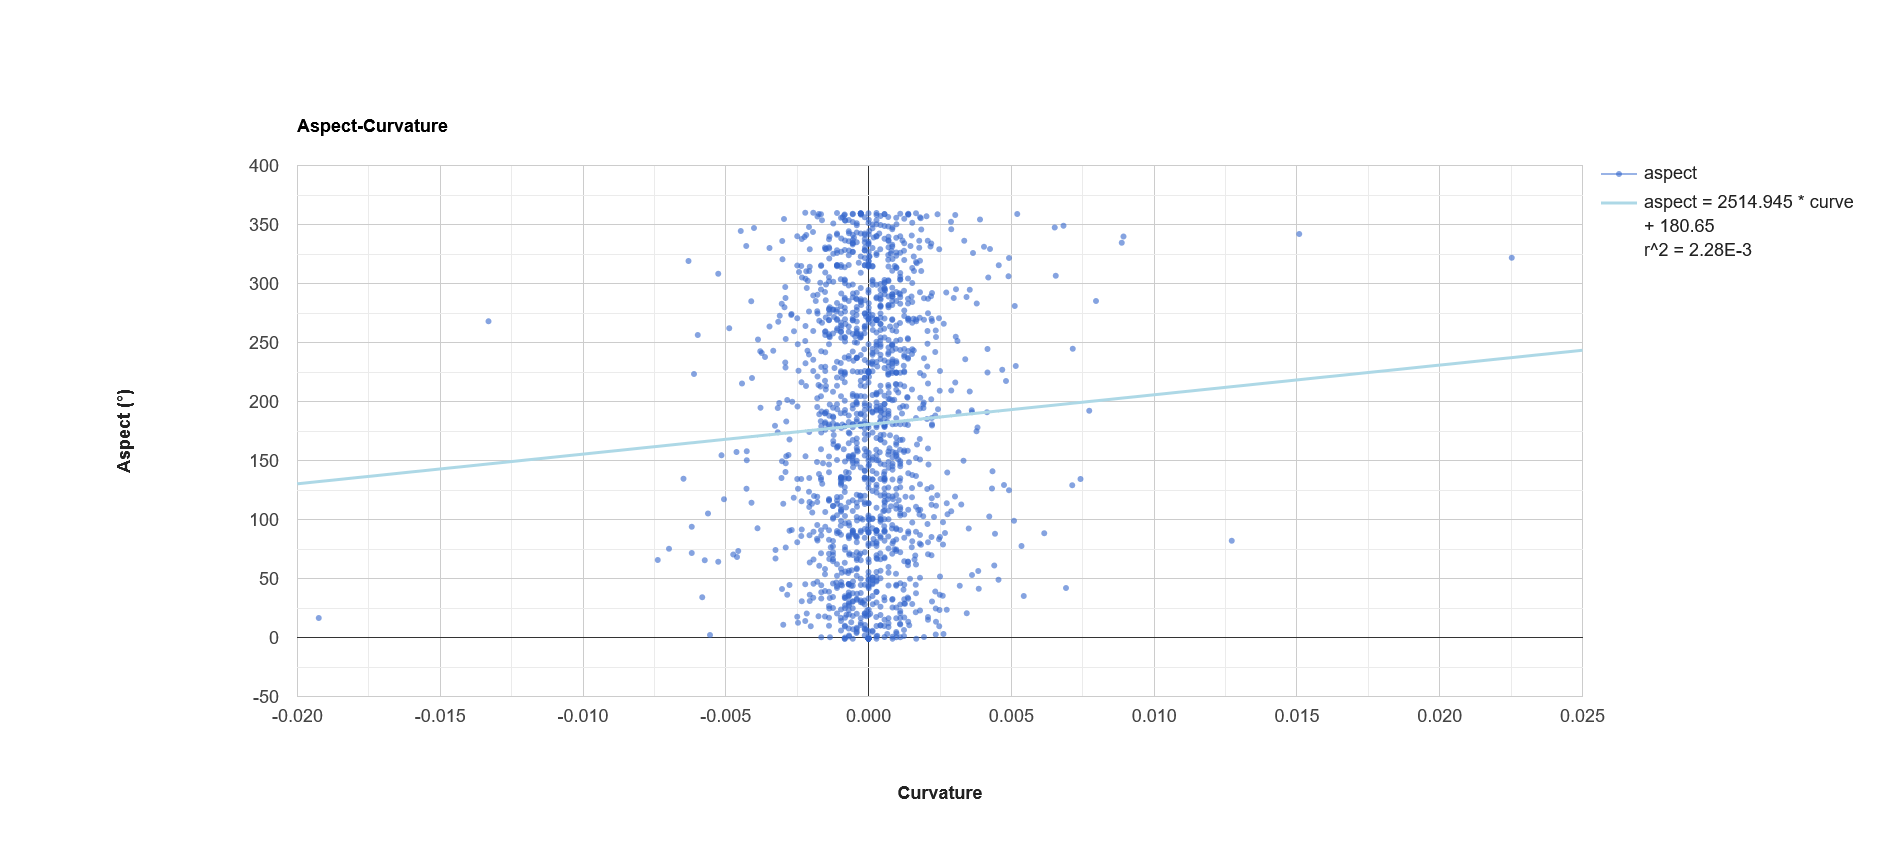
\includegraphics[keepaspectratio]{images/Collinearity/aspect-curve.png}}

}

\caption{\label{appfig-aspectCurve}Linear regression analysis of aspect
(°) and curvature for 5,000 randomly sampled points across the full
study area, encompassing Arizona.}

\end{appfig}%

\begin{appfig}

\centering{

\pandocbounded{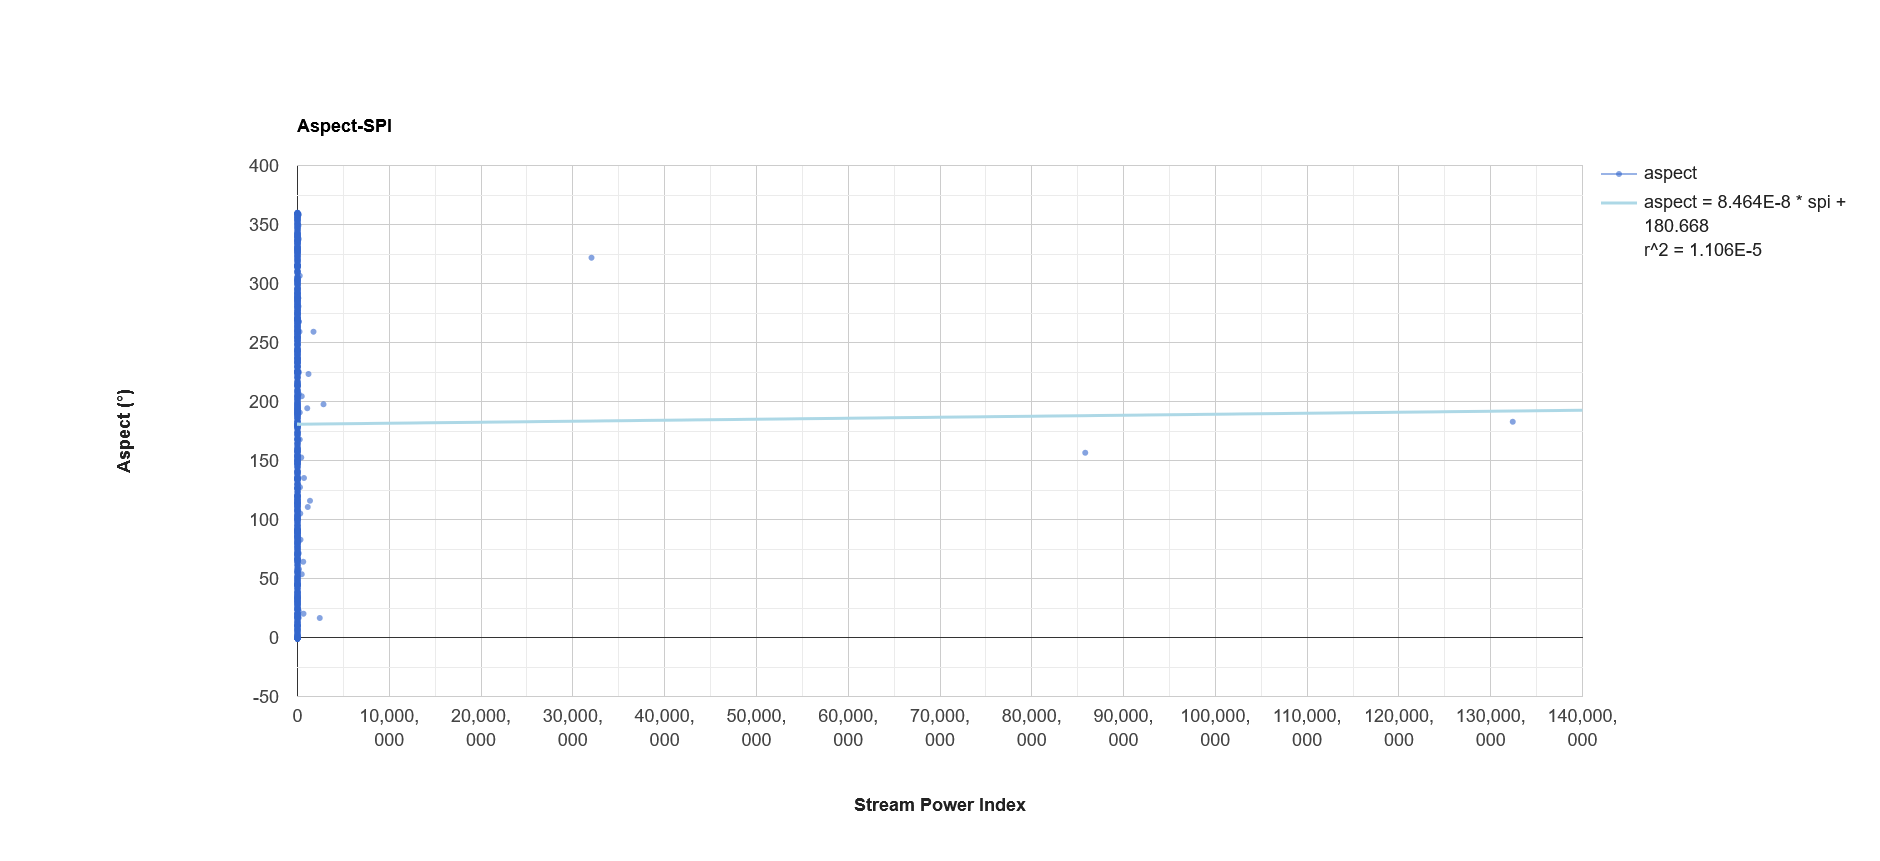
\includegraphics[keepaspectratio]{images/Collinearity/aspect-spi.png}}

}

\caption{\label{appfig-aspectSpi}Linear regression analysis of aspect
(°) and stream power index (SPI) for 5,000 randomly sampled points
across the full study area, encompassing Arizona.}

\end{appfig}%

\begin{appfig}

\centering{

\pandocbounded{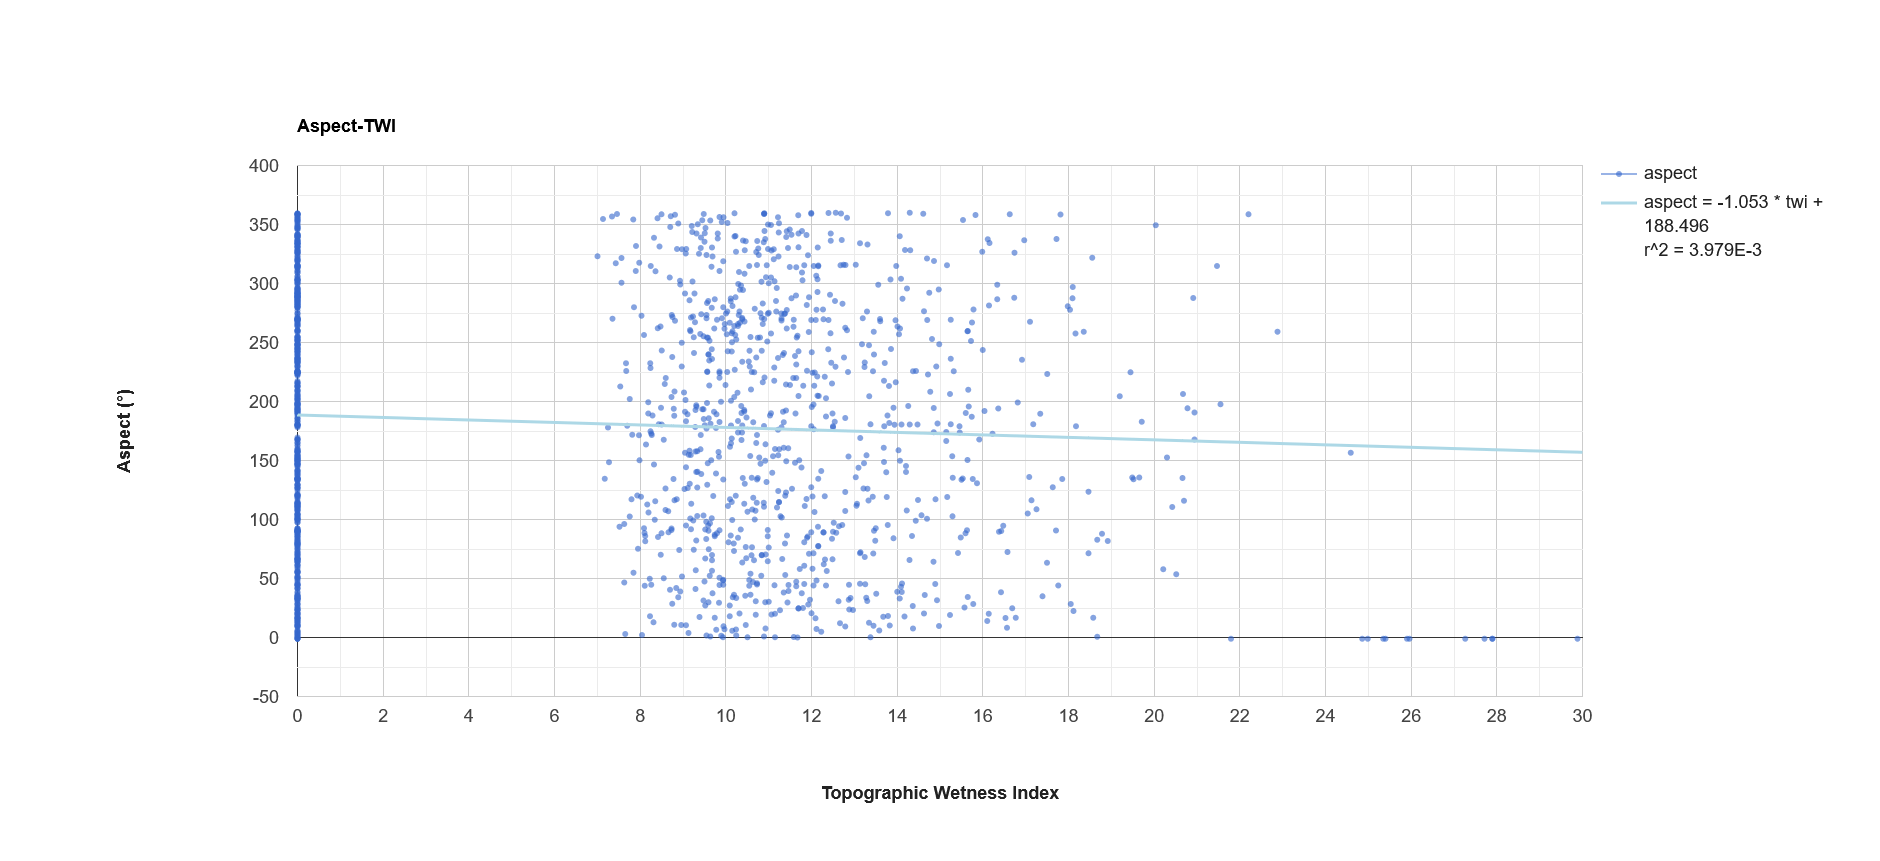
\includegraphics[keepaspectratio]{images/Collinearity/aspect-twi.png}}

}

\caption{\label{appfig-aspectTwi}Linear regression analysis of aspect
(°) and topographic wetness index (TWI) for 5,000 randomly sampled
points across the full study area, encompassing Arizona.}

\end{appfig}%

\begin{appfig}

\centering{

\pandocbounded{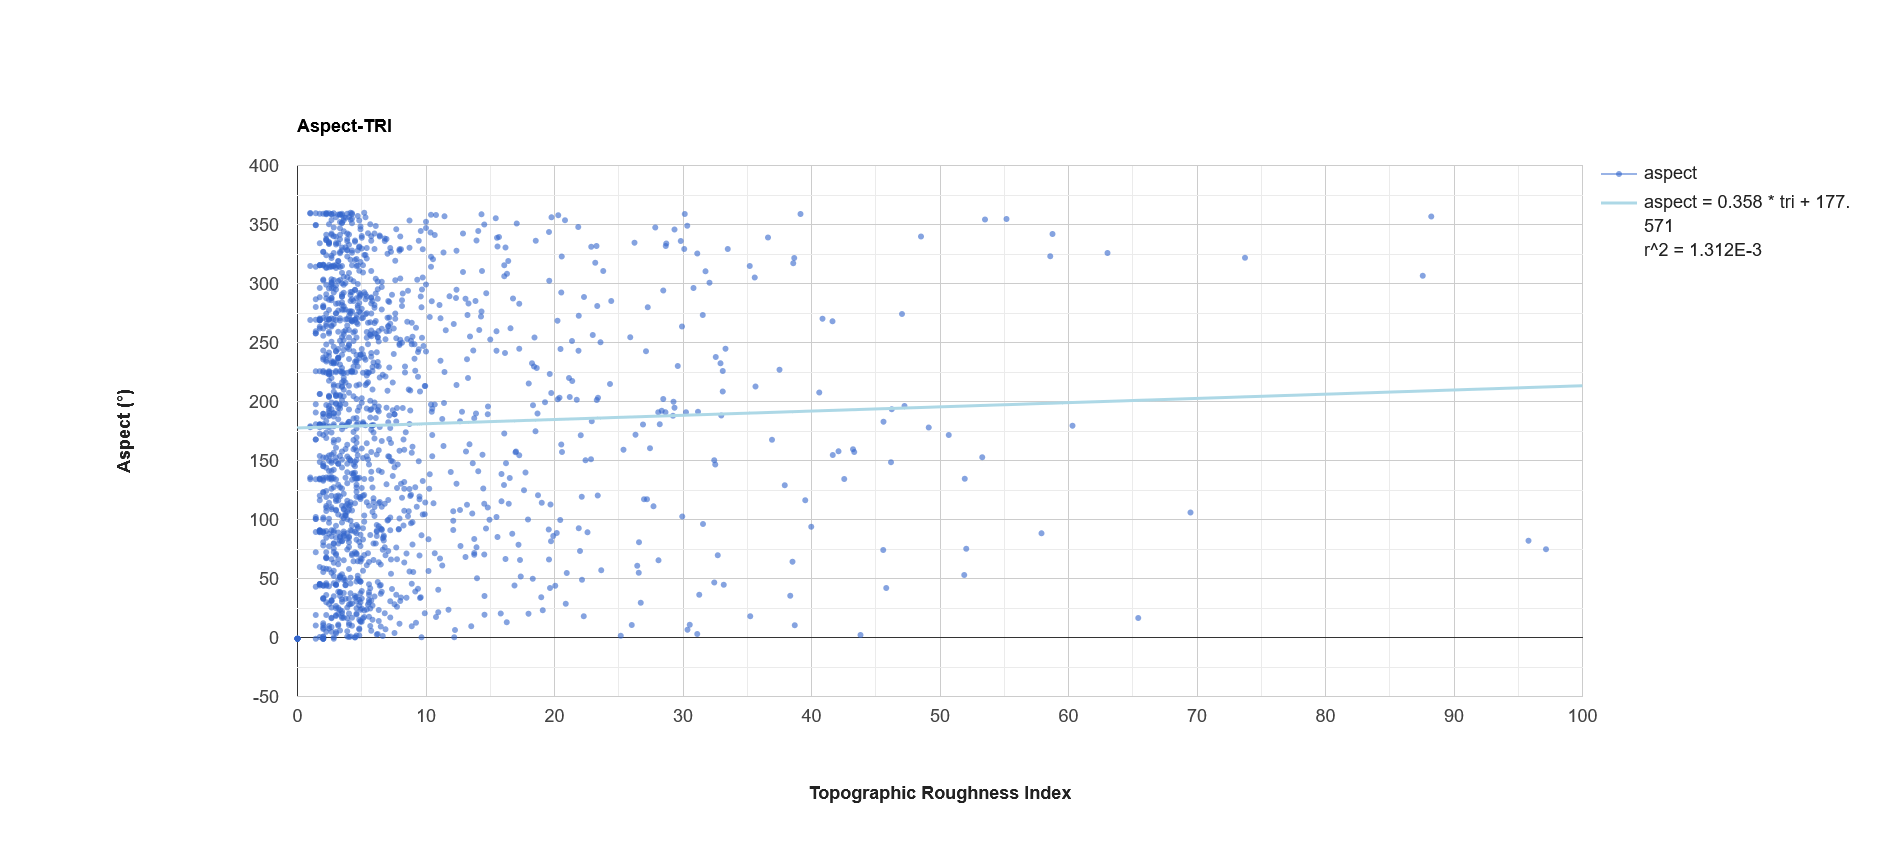
\includegraphics[keepaspectratio]{images/Collinearity/aspect-tri.png}}

}

\caption{\label{appfig-aspectTri}Linear regression analysis of aspect
(°) and topographic roughness index (TRI) for 5,000 randomly sampled
points across the full study area, encompassing Arizona.}

\end{appfig}%

\begin{appfig}

\centering{

\pandocbounded{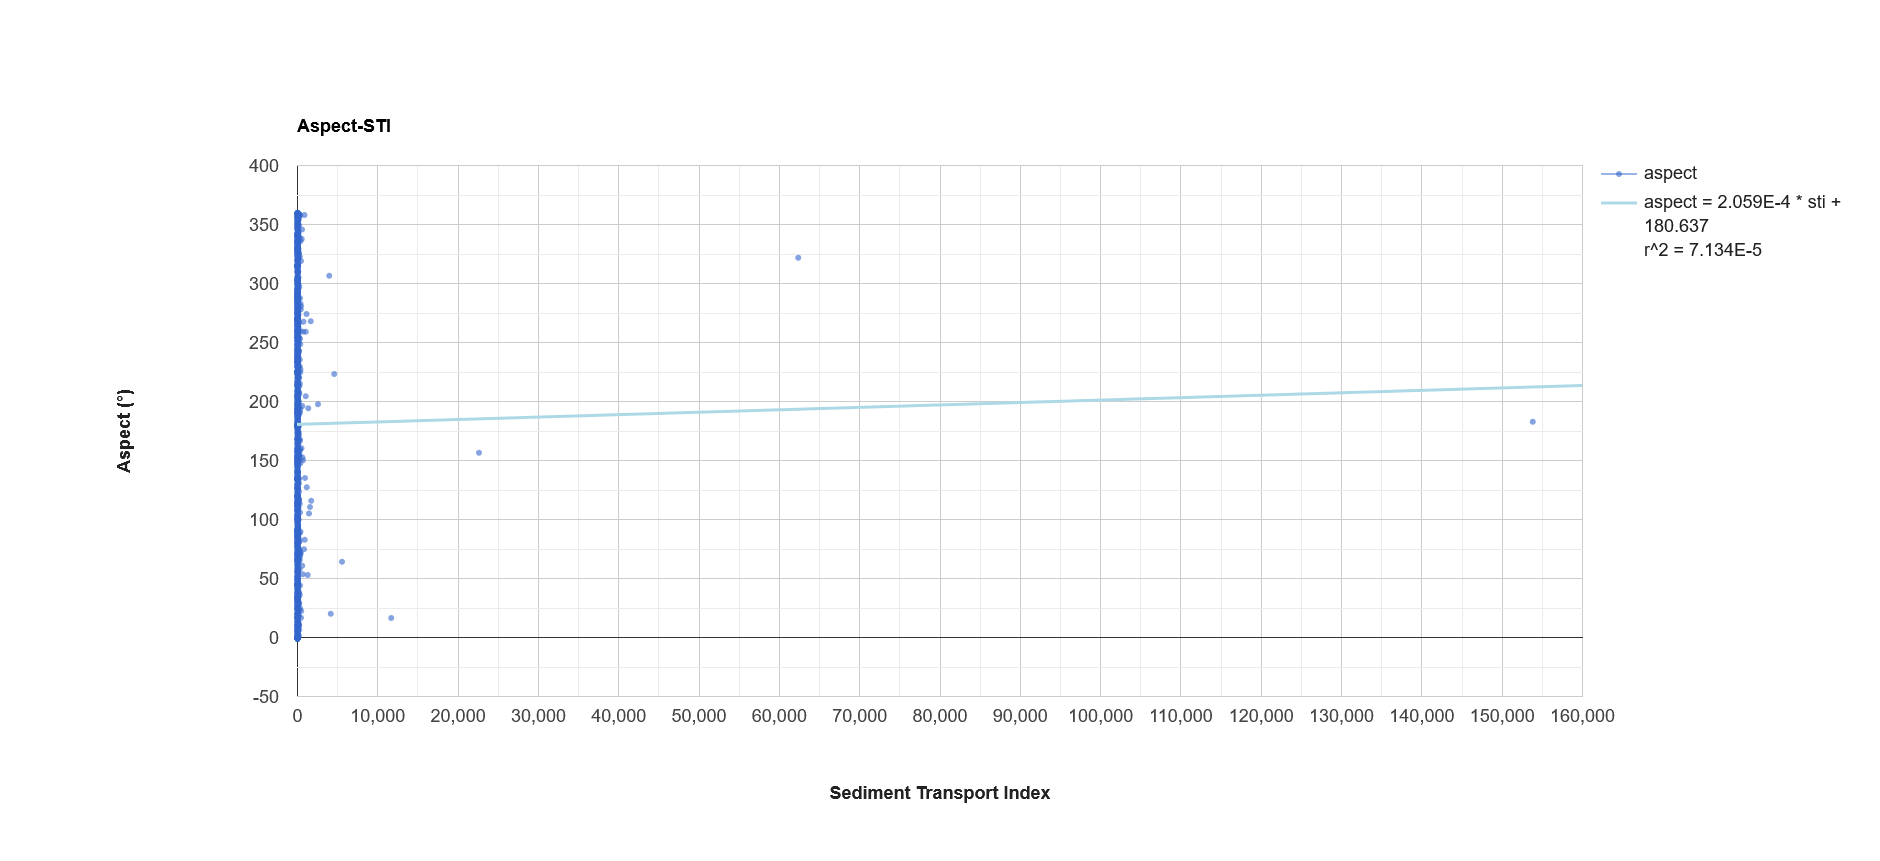
\includegraphics[keepaspectratio]{images/Collinearity/aspect-sti.png}}

}

\caption{\label{appfig-aspectSti}Linear regression analysis of aspect
(°) and sediment transport index (STI) for 5,000 randomly sampled points
across the full study area, encompassing Arizona.}

\end{appfig}%

\textbf{Curvature}

\begin{appfig}

\centering{

\pandocbounded{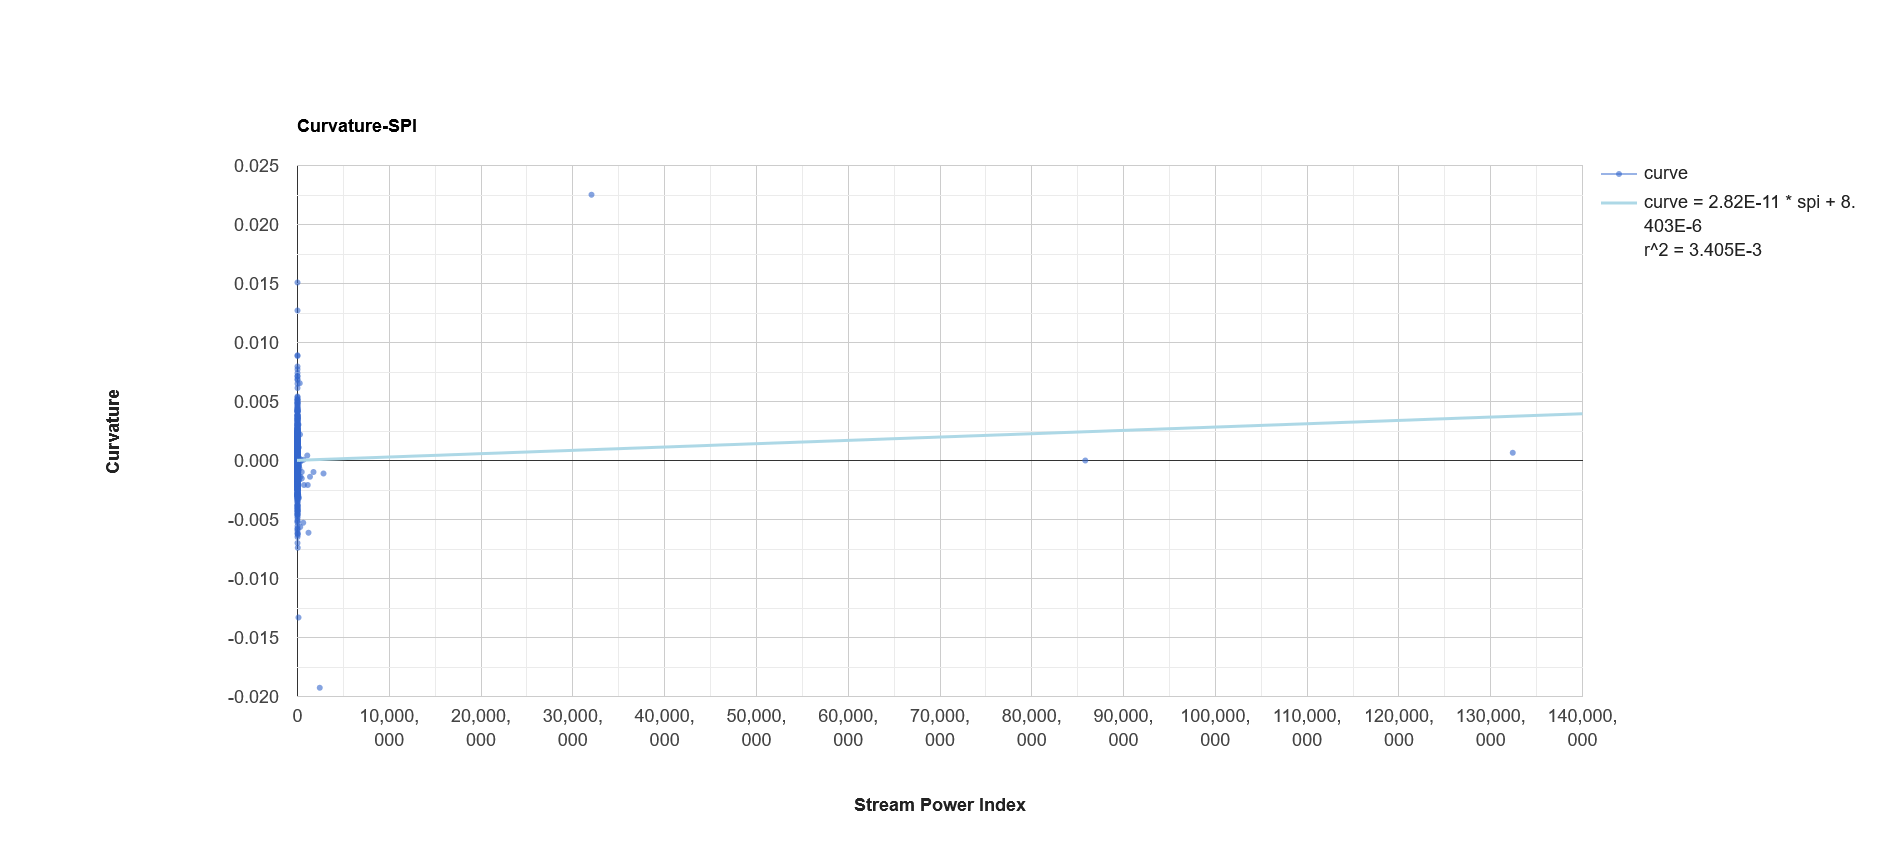
\includegraphics[keepaspectratio]{images/Collinearity/curve-spi.png}}

}

\caption{\label{appfig-curveSpi}Linear regression analysis of curvature
and stream power index (SPI) for 5,000 randomly sampled points across
the full study area, encompassing Arizona.}

\end{appfig}%

\begin{appfig}

\centering{

\pandocbounded{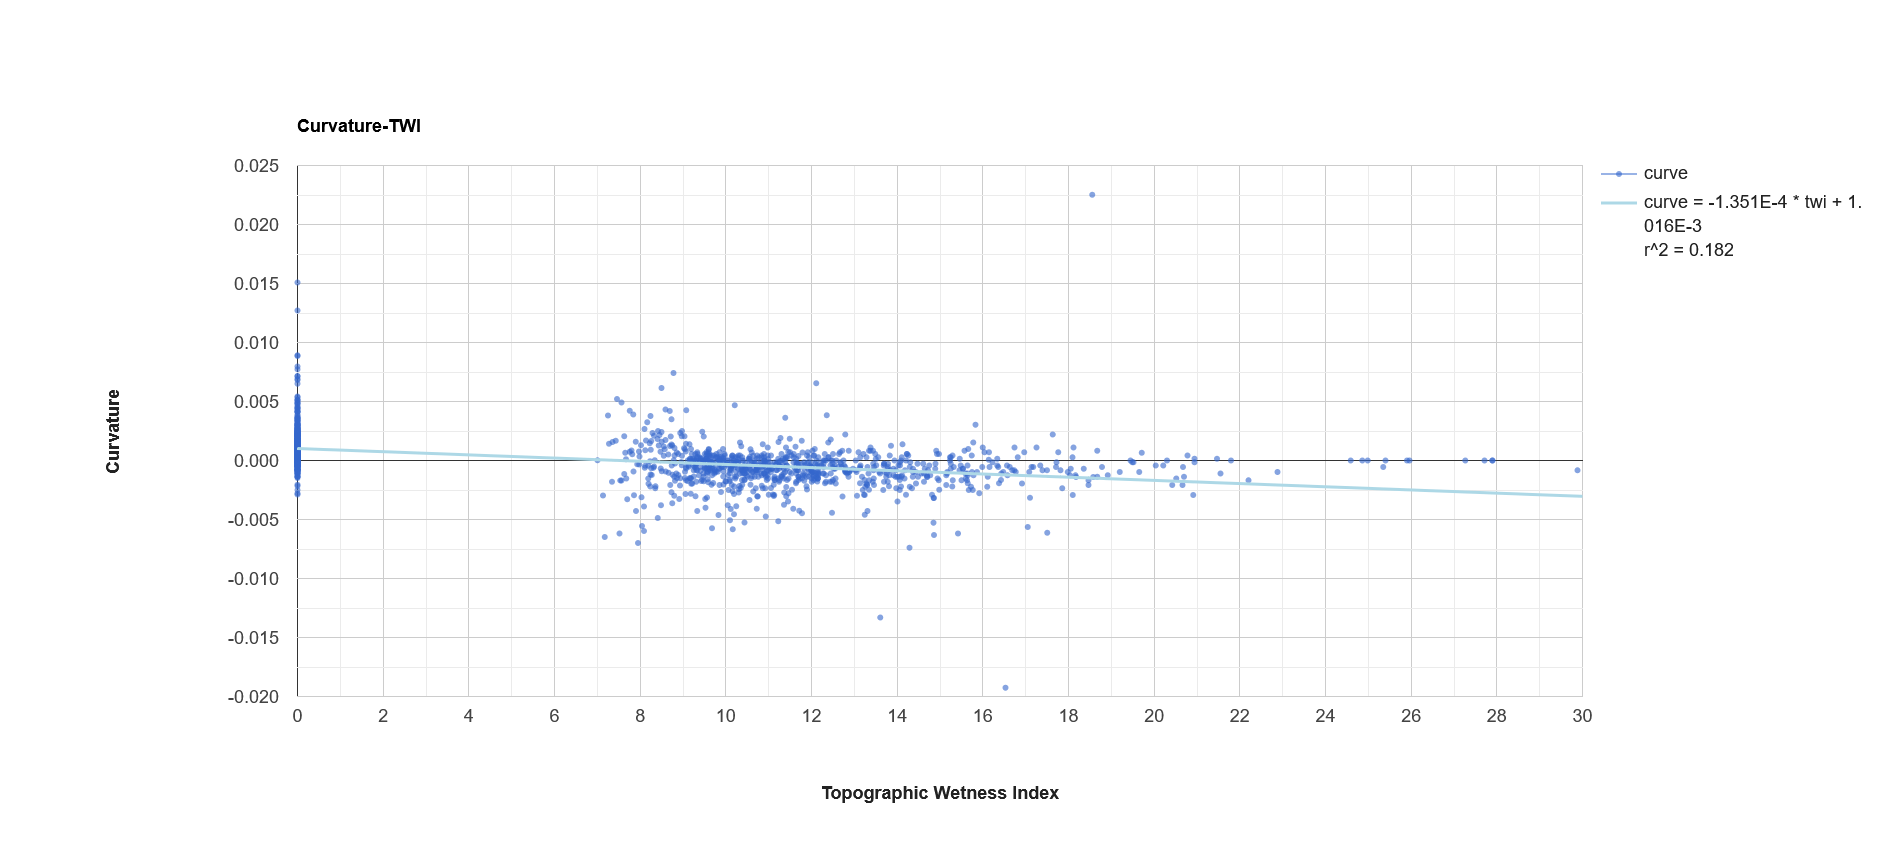
\includegraphics[keepaspectratio]{images/Collinearity/curve-twi.png}}

}

\caption{\label{appfig-curveTwi}Linear regression analysis of curvature
and topographic wetness index (TWI) for 5,000 randomly sampled points
across the full study area, encompassing Arizona.}

\end{appfig}%

\begin{appfig}

\centering{

\pandocbounded{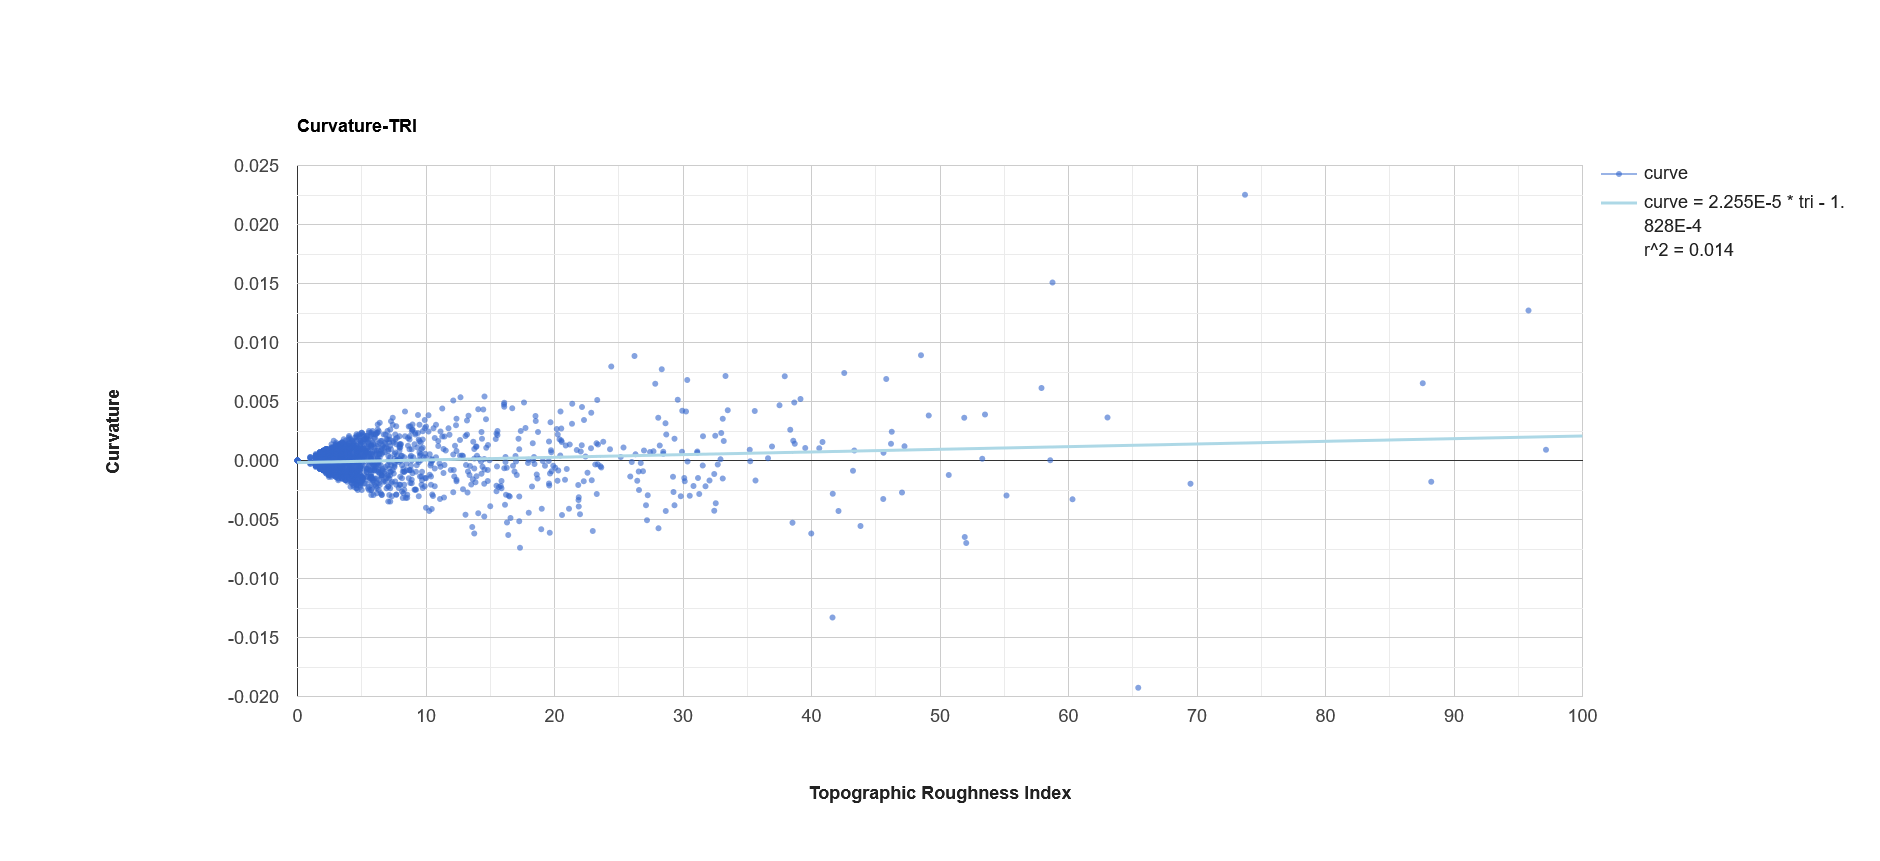
\includegraphics[keepaspectratio]{images/Collinearity/curve-tri.png}}

}

\caption{\label{appfig-curveTri}Linear regression analysis of curvature
and topographic roughness index (TRI) for 5,000 randomly sampled points
across the full study area, encompassing Arizona.}

\end{appfig}%

\begin{appfig}

\centering{

\pandocbounded{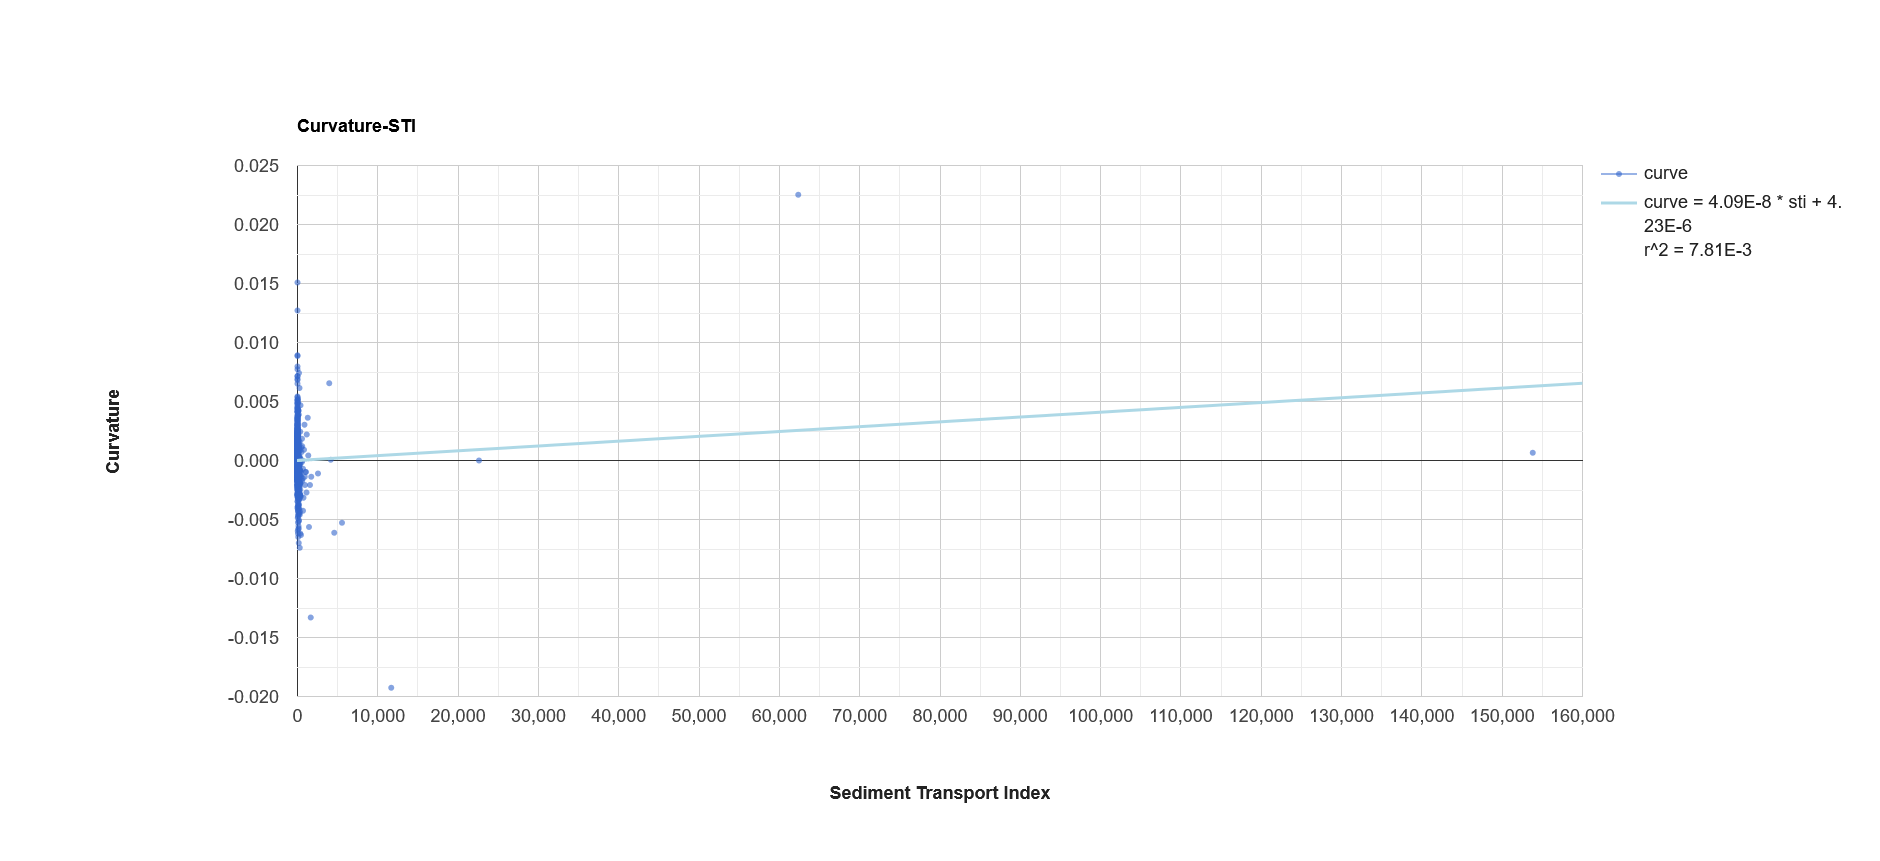
\includegraphics[keepaspectratio]{images/Collinearity/curve-sti.png}}

}

\caption{\label{appfig-curveSti}Linear regression analysis of curvature
and sediment transport index (STI) for 5,000 randomly sampled points
across the full study area, encompassing Arizona.}

\end{appfig}%

\textbf{Stream Power Index}

\begin{appfig}

\centering{

\pandocbounded{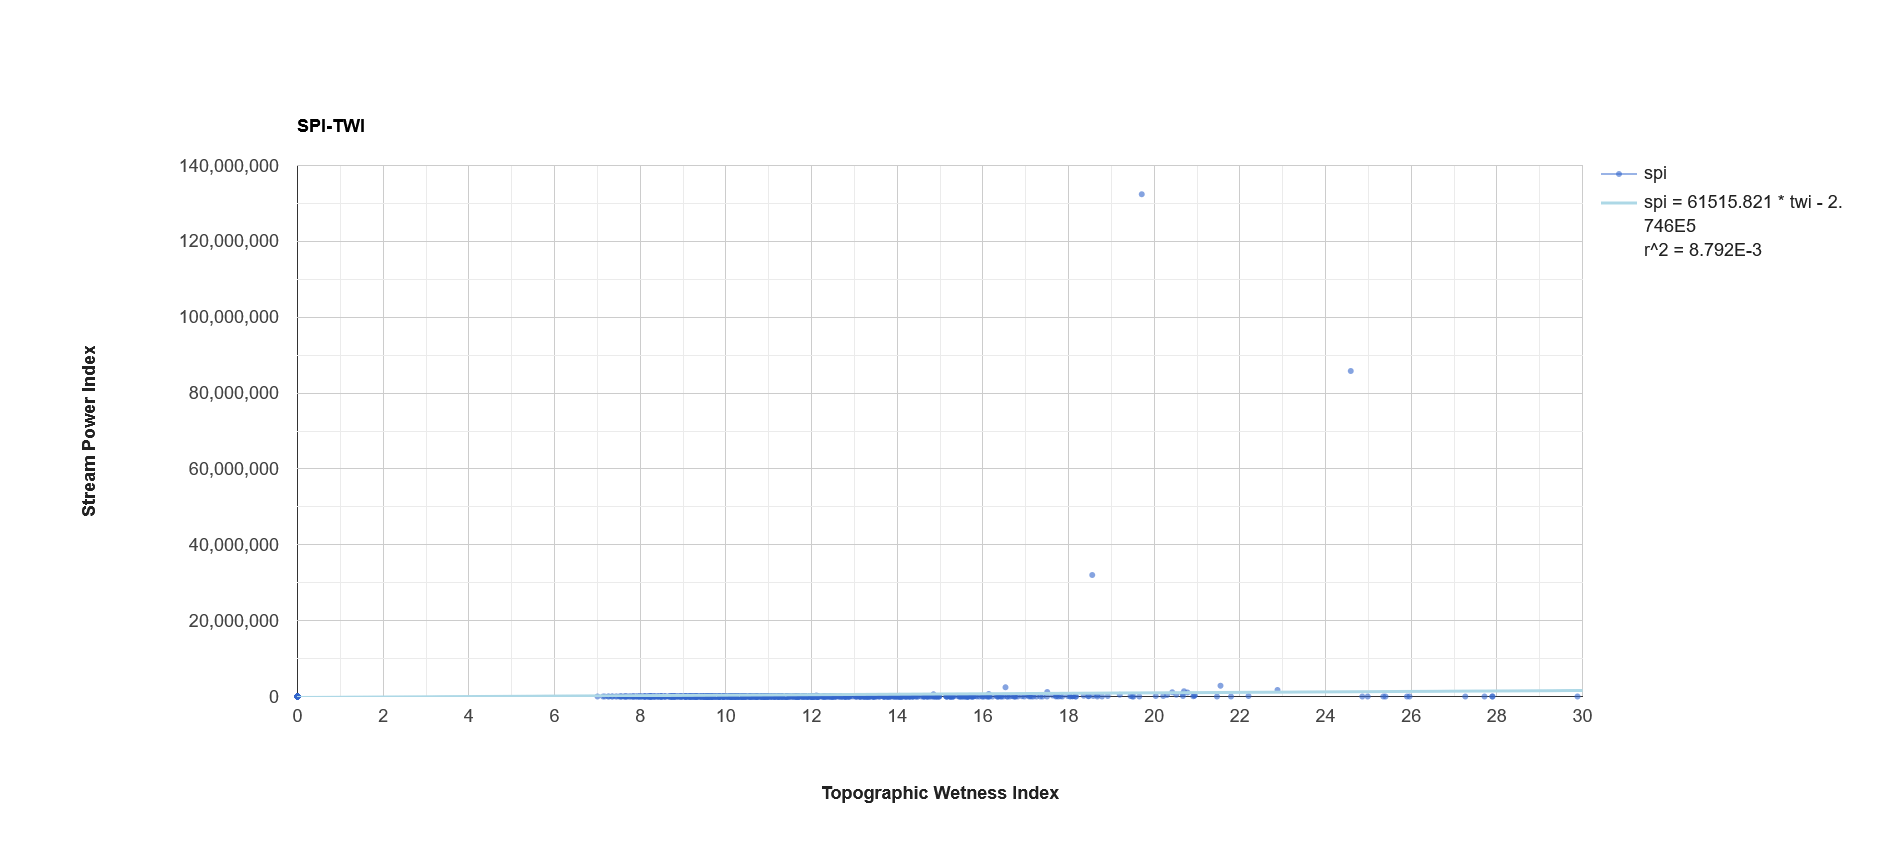
\includegraphics[keepaspectratio]{images/Collinearity/spi-twi.png}}

}

\caption{\label{appfig-spiTwi}Linear regression analysis of stream power
index (SPI) and topographic wetness index (TWI) for 5,000 randomly
sampled points across the full study area, encompassing Arizona.}

\end{appfig}%

\begin{appfig}

\centering{

\pandocbounded{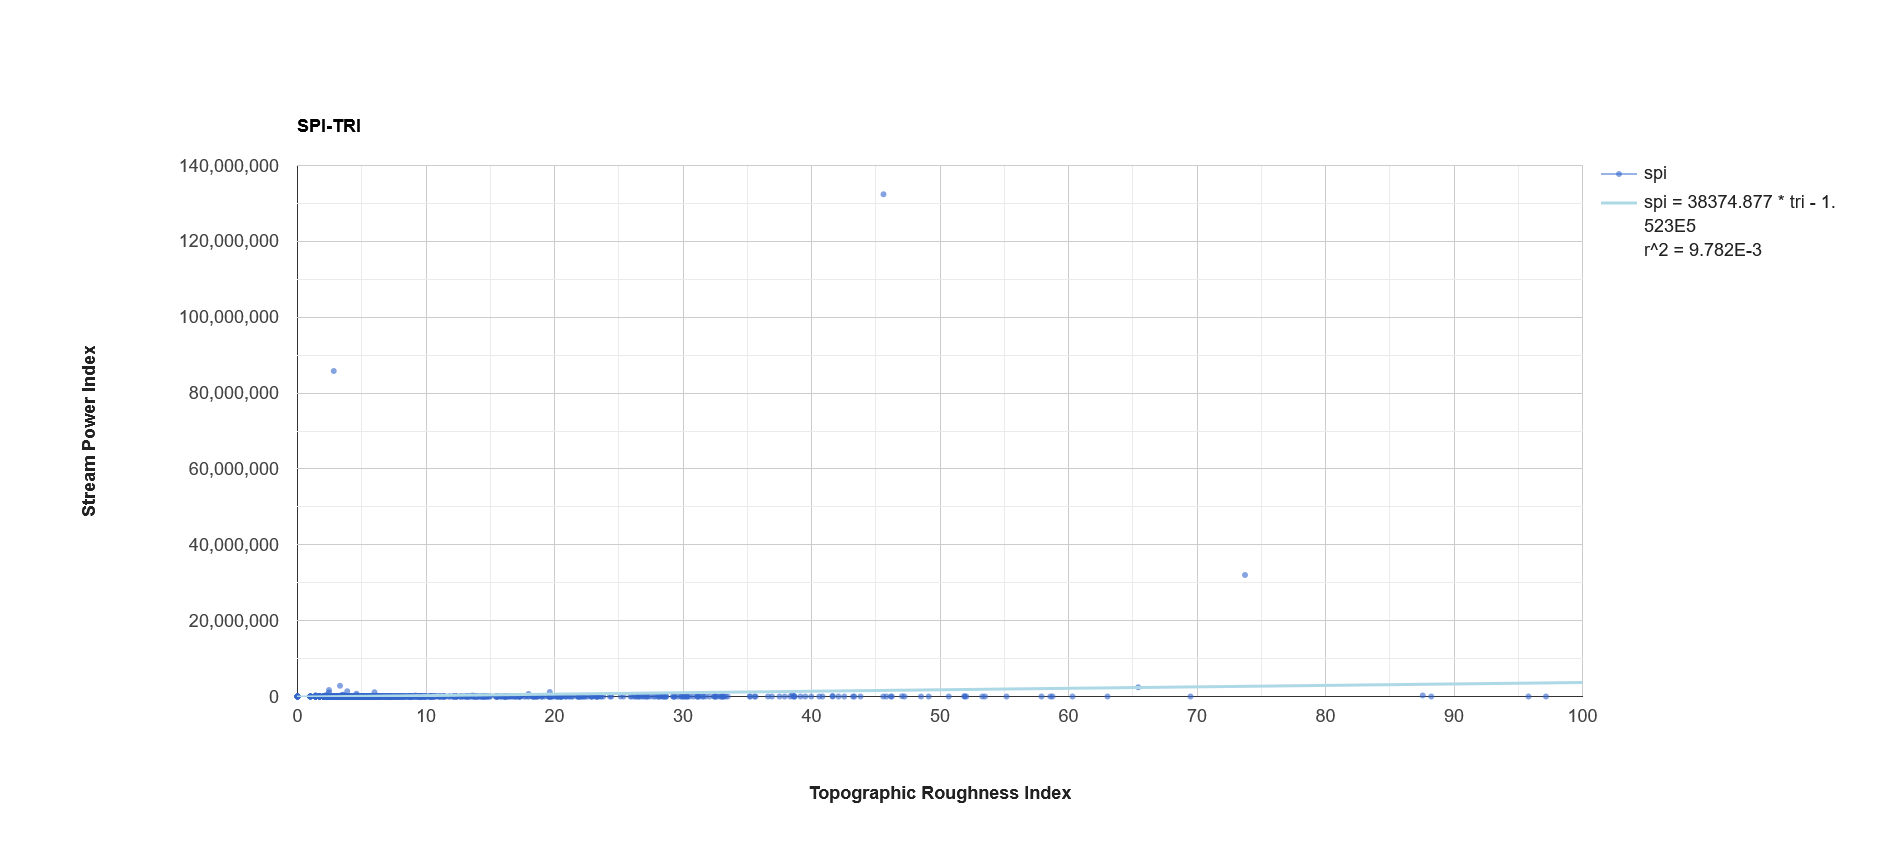
\includegraphics[keepaspectratio]{images/Collinearity/spi-tri.png}}

}

\caption{\label{appfig-spiTri}Linear regression analysis of stream power
index (SPI) and topographic roughness index (TRI) for 5,000 randomly
sampled points across the full study area, encompassing Arizona.}

\end{appfig}%

\begin{appfig}

\centering{

\pandocbounded{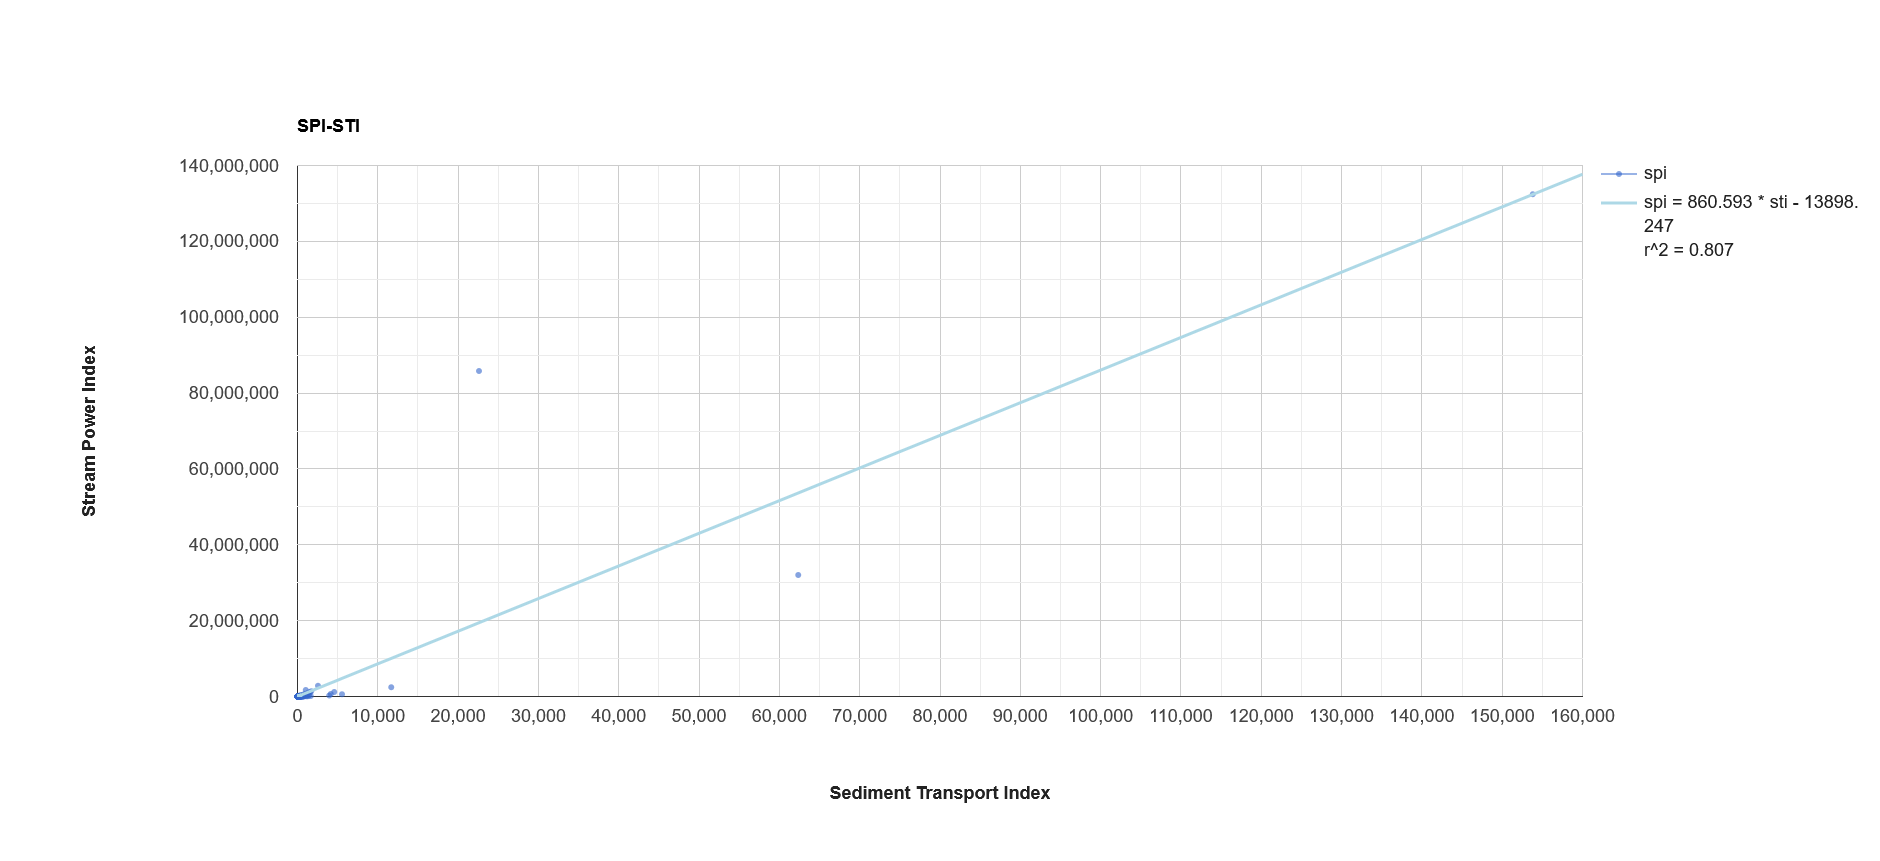
\includegraphics[keepaspectratio]{images/Collinearity/spi-sti.png}}

}

\caption{\label{appfig-spiSti}Linear regression analysis of stream power
index (SPI) and sediment transport index (STI) for 5,000 randomly
sampled points across the full study area, encompassing Arizona.}

\end{appfig}%

\textbf{Topographic Wetness Index}

\begin{appfig}

\centering{

\pandocbounded{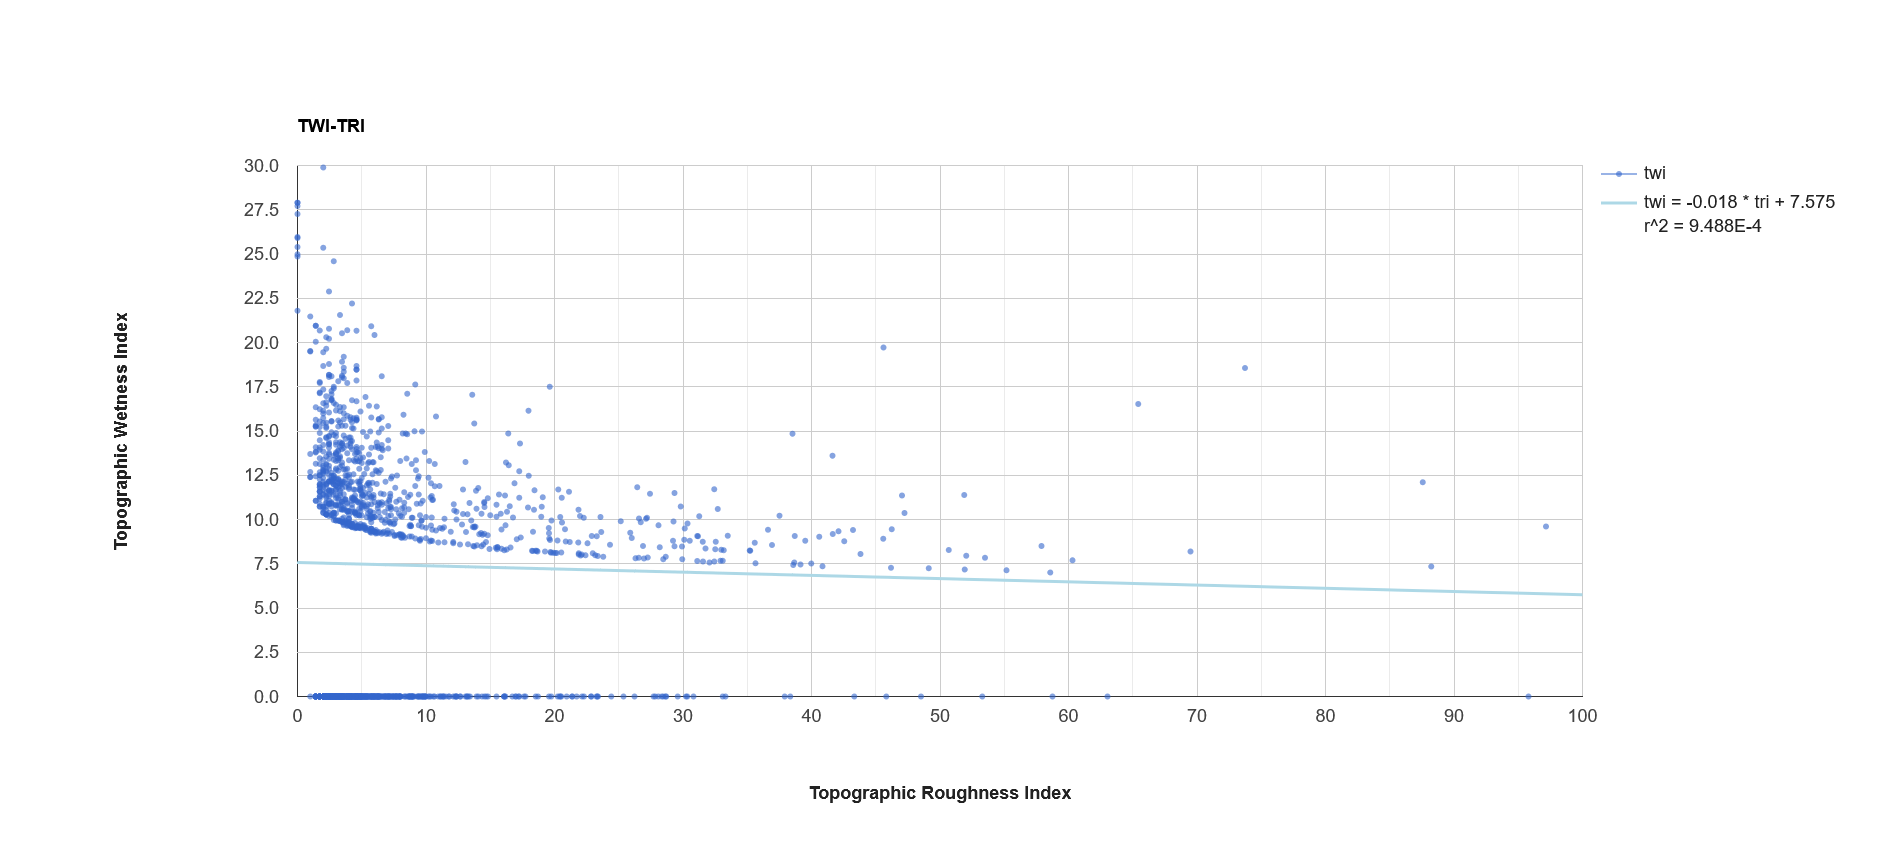
\includegraphics[keepaspectratio]{images/Collinearity/twi-tri.png}}

}

\caption{\label{appfig-twiTri}Linear regression analysis of topographic
wetness index (TWI) and topographic roughness index (TRI) for 5,000
randomly sampled points across the full study area, encompassing
Arizona.}

\end{appfig}%

\begin{appfig}

\centering{

\pandocbounded{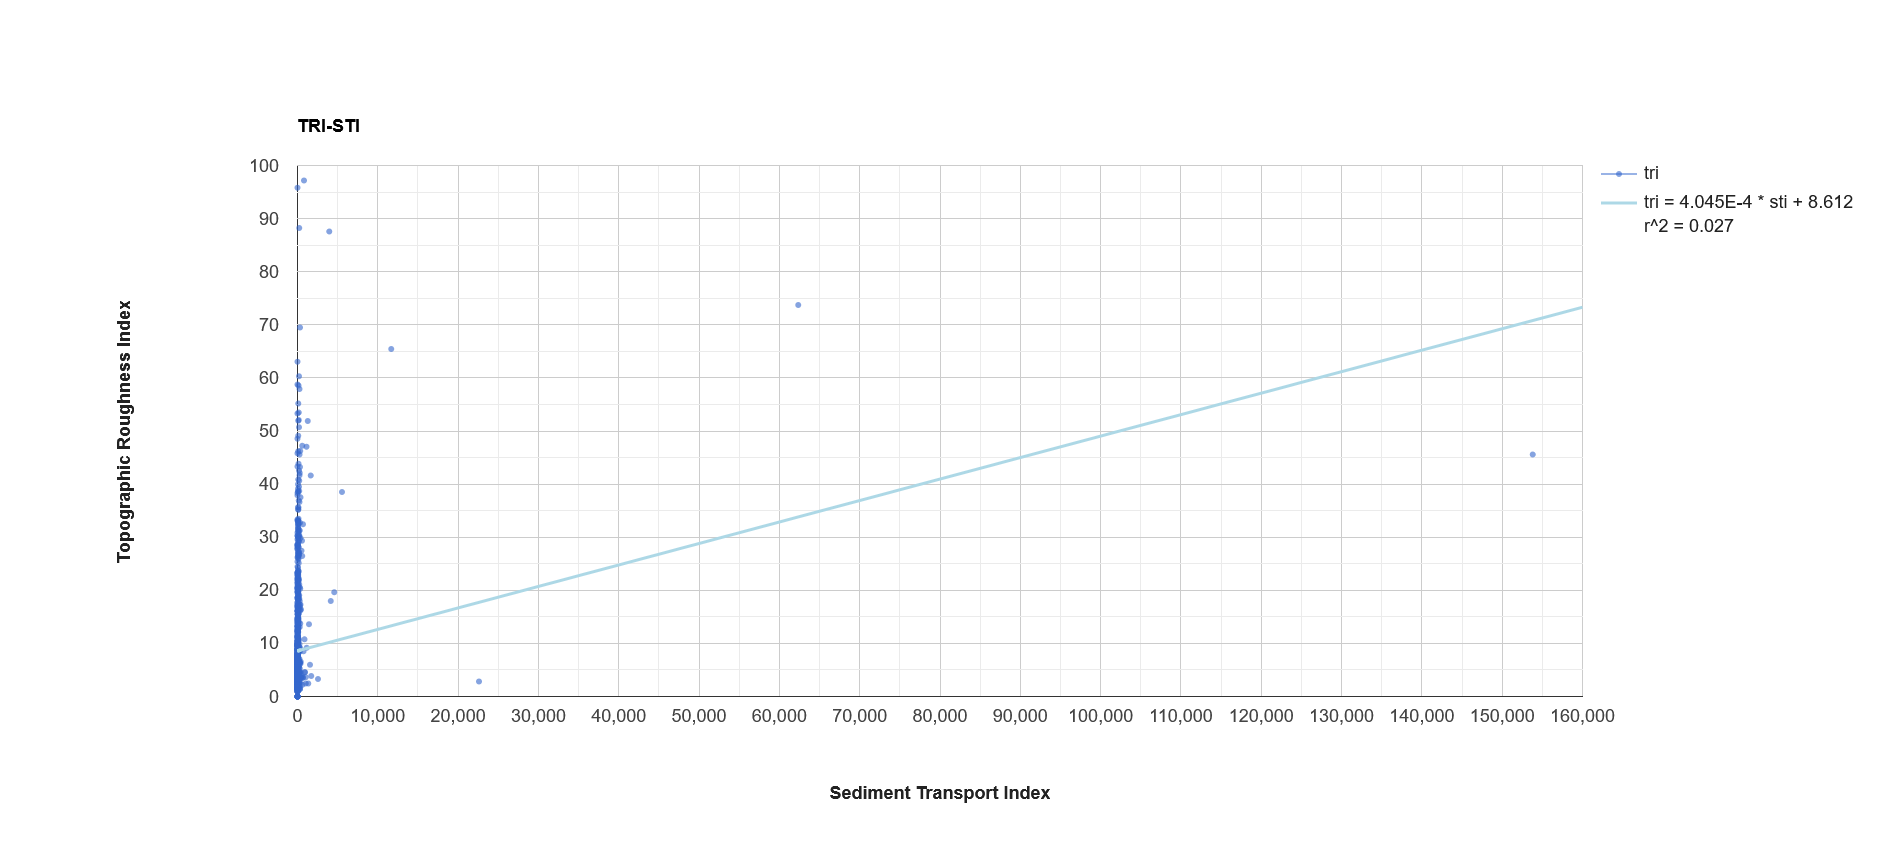
\includegraphics[keepaspectratio]{images/Collinearity/tri-sti.png}}

}

\caption{\label{appfig-twiSti}Linear regression analysis of topographic
wetness index (TRI) and sediment transport index (STI) for 5,000
randomly sampled points across the full study area, encompassing
Arizona.}

\end{appfig}%

\textbf{Topographic Roughness Index}

\begin{appfig}

\centering{

\pandocbounded{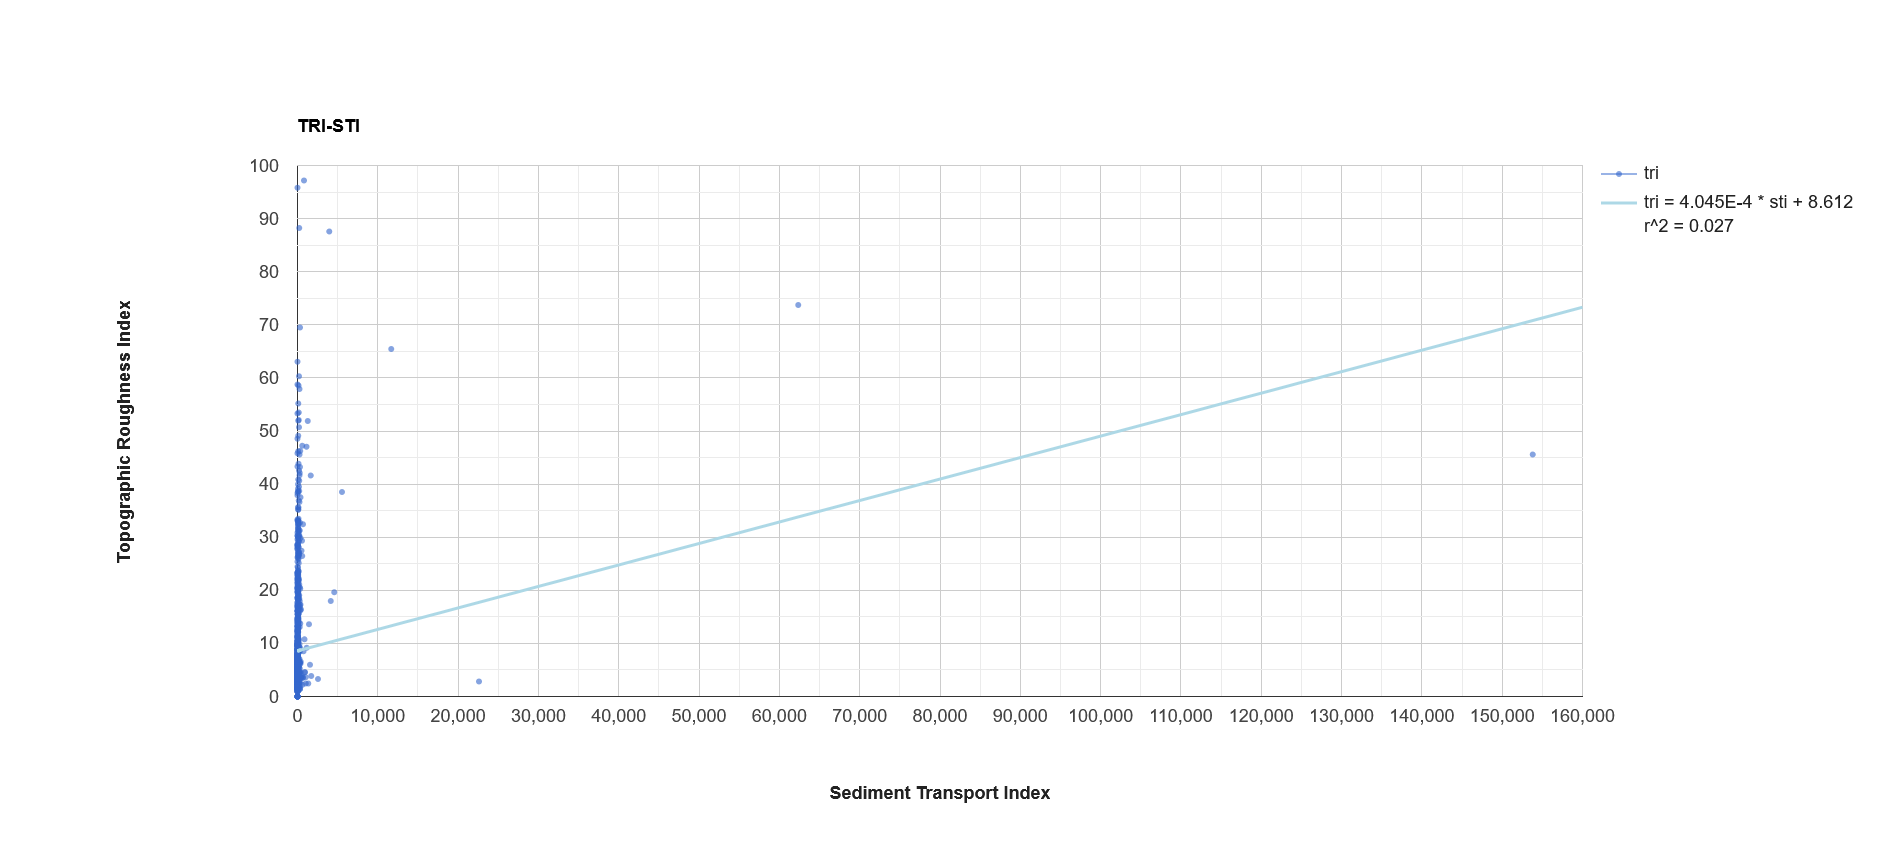
\includegraphics[keepaspectratio]{images/Collinearity/tri-sti.png}}

}

\caption{\label{appfig-triSti}Linear regression analysis of topographic
roughness index (TRI) and sediment transport index (STI) for 5,000
randomly sampled points across the full study area, encompassing
Arizona.}

\end{appfig}%




\end{document}
